\documentclass{mimosis}

\usepackage{metalogo}
\usepackage{xargs} % Use more than one optional parameter in a new commands
\usepackage{indentfirst}

\usepackage[colorinlistoftodos,prependcaption,textsize=tiny]{todonotes}
\newcommandx{\unsure}[2][1=]{\todo[linecolor=red,backgroundcolor=red!25,bordercolor=red,#1]{#2}}
\newcommandx{\change}[2][1=]{\todo[linecolor=blue,backgroundcolor=blue!25,bordercolor=blue,#1]{#2}}

\newcommandx{\info}[2][1=]{\todo[linecolor=OliveGreen,backgroundcolor=OliveGreen!25,bordercolor=OliveGreen,#1]{#2}}
\newcommandx{\improvement}[2][1=]{\todo[linecolor=Plum,backgroundcolor=Plum!25,bordercolor=Plum,#1]{#2}}
\newcommandx{\thiswillnotshow}[2][1=]{\todo[disable,#2]{#1}}
%

\usepackage{float}
\usepackage{geometry}
\usepackage{babel}
\usepackage{booktabs}
\newcommand{\ra}[1]{\renewcommand{\arraystretch}{#1}}

\graphicspath{ {./img/} }

\newcommand{\alphabet}{%
  abcdefghijklmnopqrstuvwxyz%
}
\newlength{\textW}
\setlength{\textW}{\widthof{\alphabet}* \real{2.8}} % 2.5
\geometry{textwidth=\textW,}
\newcommand{\myref}[2]{\hyperref[#2]{#1~\ref*{#2}}}
%%%%%%%%%%%%%%%%%%%%%%%%%%%%%%%%%%%%%%%%%%%%%%%%%%%%%%%%%%%%%%%%%%%%%%%%
% Some of my favourite personal adjustments
%%%%%%%%%%%%%%%%%%%%%%%%%%%%%%%%%%%%%%%%%%%%%%%%%%%%%%%%%%%%%%%%%%%%%%%%
%
% These are the adjustments that I consider necessary for typesetting
% a nice thesis. However, they are *not* included in the template, as
% I do not want to force you to use them.

% This ensures that I am able to typeset bold font in table while still aligning the numbers
% correctly.
\usepackage{etoolbox}
\usepackage{listings}

\usepackage[binary-units=true]{siunitx}
\DeclareSIUnit\px{px}

\sisetup{%
  detect-all           = true,
  detect-family        = true,
  detect-mode          = true,
  detect-shape         = true,
  detect-weight        = true,
  detect-inline-weight = math,
}

%%%%%%%%%%%%%%%%%%%%%%%%%%%%%%%%%%%%%%%%%%%%%%%%%%%%%%%%%%%%%%%%%%%%%%%%
% Hyperlinks & bookmarks
%%%%%%%%%%%%%%%%%%%%%%%%%%%%%%%%%%%%%%%%%%%%%%%%%%%%%%%%%%%%%%%%%%%%%%%%

\usepackage[%
  colorlinks = true,
  citecolor  = OliveGreen,
  linkcolor  = Mahogany,
  urlcolor   = RoyalBlue,
  unicode,
  ]{hyperref}


\newcommand{\smallquote}[1]{
    \begin{center}
        \begin{minipage}{0.5\textwidth}
            \begin{small}
                #1
            \end{small}
        \end{minipage}
        \vspace{0.5cm}
    \end{center}
}

\usepackage{bookmark}

\usepackage[all]{nowidow}

%%%%%%%%%%%%%%%%%%%%%%%%%%%%%%%%%%%%%%%%%%%%%%%%%%%%%%%%%%%%%%%%%%%%%%%%
% Bibliography
%%%%%%%%%%%%%%%%%%%%%%%%%%%%%%%%%%%%%%%%%%%%%%%%%%%%%%%%%%%%%%%%%%%%%%%%
%
% I like the bibliography to be extremely plain, showing only a numeric
% identifier and citing everything in simple brackets. The first names,
% if present, will be initialized. DOIs and URLs will be preserved.

\usepackage[%
  autocite     = plain,
  backend      = biber,
  doi          = true,
  url          = true,
  giveninits   = true,
  hyperref     = true,
  maxbibnames  = 99,
  maxcitenames = 99,
  sortcites    = true,
  style        = iso-numeric,
  ]{biblatex}

%%%%%%%%%%%%%%%%%%%%%%%%%%%%%%%%%%%%%%%%%%%%%%%%%%%%%%%%%%%%%%%%%%%%%%%%
% Some adjustments to make the bibliography more clean
%%%%%%%%%%%%%%%%%%%%%%%%%%%%%%%%%%%%%%%%%%%%%%%%%%%%%%%%%%%%%%%%%%%%%%%%
%
% The subsequent commands do the following:
%  - Removing the month field from the bibliography
%  - Fixing the Oxford commma
%  - Suppress the "in" for journal articles
%  - Remove the parentheses of the year in an article
%  - Delimit volume and issue of an article by a colon ":" instead of
%    a dot ""
%  - Use commas to separate the location of publishers from their name
%  - Remove the abbreviation for technical reports
%  - Display the label of bibliographic entries without brackets in the
%    bibliography
%  - Ensure that DOIs are followed by a non-breakable space
%  - Use hair spaces between initials of authors
%  - Make the font size of citations smaller
%  - Fixing ordinal numbers (1st, 2nd, 3rd, and so) on by using
%    superscripts

% Remove the month field from the bibliography. It does not serve a good
% purpose, I guess. And often, it cannot be used because the journals
% have some crazy issue policies.
\AtEveryBibitem{\clearfield{month}}
\AtEveryCitekey{\clearfield{month}}

% Fixing the Oxford comma. Not sure whether this is the proper solution.
% More information is available under [1] and [2].
%
% [1] http://tex.stackexchange.com/questions/97712/biblatex-apa-style-is-missing-a-comma-in-the-references-why
% [2] http://tex.stackexchange.com/questions/44048/use-et-al-in-biblatex-custom-style
%
\AtBeginBibliography{%
  \renewcommand*{\finalnamedelim}{%
    \ifthenelse{\value{listcount} > 2}{%
      \addcomma
      \addspace
      \bibstring{and}%
    }{%
      \addspace
      \bibstring{and}%
    }
  }
}

% Suppress "in" for journal articles. This is unnecessary in my opinion
% because the journal title is typeset in italics anyway.
\renewbibmacro{in:}{%
  \ifentrytype{article}
  {%
  }%
  % else
  {%
    \printtext{\bibstring{in}\intitlepunct}%
  }%
}

% Remove the parentheses for the year in an article. This removes a lot
% of undesired parentheses in the bibliography, thereby improving the
% readability. Moreover, it makes the look of the bibliography more
% consistent.
\renewbibmacro*{issue+date}{%
  \setunit{\addcomma\space}
    \iffieldundef{issue}
      {\usebibmacro{date}}
      {\printfield{issue}%
       \setunit*{\addspace}%
       \usebibmacro{date}}%
  \newunit}

% Delimit the volume and the number of an article by a colon instead of
% by a dot, which I consider to be more readable.
\renewbibmacro*{volume+number+eid}{%
  \printfield{volume}%
  \setunit*{\addcolon}%
  \printfield{number}%
  \setunit{\addcomma\space}%
  \printfield{eid}%
}

% Do not use a colon for the publisher location. Instead, connect
% publisher, location, and date via commas.
\renewbibmacro*{publisher+location+date}{%
  \printlist{publisher}%
  \setunit*{\addcomma\space}%
  \printlist{location}%
  \setunit*{\addcomma\space}%
  \usebibmacro{date}%
  \newunit%
}

% Ditto for other entry types.
\renewbibmacro*{organization+location+date}{%
  \printlist{location}%
  \setunit*{\addcomma\space}%
  \printlist{organization}%
  \setunit*{\addcomma\space}%
  \usebibmacro{date}%
  \newunit%
}

% Display the label of a bibliographic entry in bare style, without any
% brackets. I like this more than the default.
%
% Note that this is *really* the proper and official way of doing this.
\DeclareFieldFormat{labelnumberwidth}{#1\adddot}

% Ensure that DOIs are followed by a non-breakable space.
\DeclareFieldFormat{doi}{%
  \mkbibacro{DOI}\addcolon\addnbspace
    \ifhyperref
      {\href{http://dx.doi.org/#1}{\nolinkurl{#1}}}
      %
      {\nolinkurl{#1}}
}

\DefineBibliographyStrings{english}{
  online = {online}
}

\DefineBibliographyStrings{english}{
  urlalso = {Available from}
}


% Use proper hair spaces between initials as suggested by Bringhurst and
% others.
\renewcommand*\bibinitdelim {\addnbthinspace}
\renewcommand*\bibnamedelima{\addnbthinspace}
\renewcommand*\bibnamedelimb{\addnbthinspace}
\renewcommand*\bibnamedelimi{\addnbthinspace}

% Make the font size of citations smaller. Depending on your selected
% font, you might not need this.
\renewcommand*{\citesetup}{%
  \biburlsetup
  \small
}

\DeclareLanguageMapping{english}{english-mimosis}

\addbibresource{Thesis.bib}

%%%%%%%%%%%%%%%%%%%%%%%%%%%%%%%%%%%%%%%%%%%%%%%%%%%%%%%%%%%%%%%%%%%%%%%%
% Fonts
%%%%%%%%%%%%%%%%%%%%%%%%%%%%%%%%%%%%%%%%%%%%%%%%%%%%%%%%%%%%%%%%%%%%%%%%

\ifxetexorluatex
  % \setmainfont{Minion Pro}
    \setmainfont{Baskerville}
    \setsansfont{IBM Plex Sans}
    \setmonofont{IBM Plex Mono}
\else
  \usepackage[lf]{ebgaramond}
  \usepackage[oldstyle,scale=0.7]{sourcecodepro}
  \singlespacing
\fi

\renewcommand{\th}{\textsuperscript{\textup{th}}\xspace}

\newacronym{CAM}{CAM}{Class Activation Map}
\newacronym{DL}{DL}{Deep Learning}
\newacronym{LRP}{LRP}{Layer-Wise Relevance Propagation}
\newacronym{XAI}{XAI}{Explainable Artificial Intelligence}

\usepackage{textcomp}

\makeindex
\makeglossaries

%%%%%%%%%%%%%%%%%%%%%%%%%%%%%%%%%%%%%%%%%%%%%%%%%%%%%%%%%%%%%%%%%%%%%%%%
% Incipit
%%%%%%%%%%%%%%%%%%%%%%%%%%%%%%%%%%%%%%%%%%%%%%%%%%%%%%%%%%%%%%%%%%%%%%%%

\title{Effectiveness of Interpretation Techniques For Deep Networks in Digital Histopathology}
\author{Martin Krebs}

% This ensures that the subsequent sections are being included as root
% items in the bookmark structure of your PDF reader.
\begin{document}
\frontmatter
    \begin{titlepage}
  \vspace*{2cm}
  \makeatletter
  \begin{center}
      \begin{LARGE}
          \textsc{Masaryk University}
      \end{LARGE}\\[0.01cm]
      \begin{Large}
          \textsc{Faculty of Informatics\\}
      \end{Large}
      \vspace*{1cm}
      \includegraphics[width=40mm]{fithesis-fi.pdf}\\
      \vspace*{3cm}
    \begin{Huge}
      \@title
    \end{Huge}\\[1.5cm]
    %
    \begin{Large}
        \textsc{Bachelor's Thesis}
    \end{Large}\\[1.5cm]
    %
    \begin{LARGE}
        \@author
    \end{LARGE}
    %
    \vfill
  \end{center}
  \begin{flushright}
      \begin{large}
        Brno, Spring 2024
      \end{large}
  \end{flushright}
  \makeatother
\end{titlepage}

\newpage
\null
\thispagestyle{empty}
\newpage

    \chapter*{Declaration}

\noindent
Hereby I declare, that this paper is my original authorial work, which I have worked out on my own.
All sources, references, and literature used or excerpted during the elaboration of this work are properly cited and listed in complete reference to the due source.

While preparing this thesis, I used Grammarly to improve my writing style and grammar.
I used ChatGPT by OpenAI to help me generate code for graph visualizations and express myself in places where my thoughts were too tangled.
I declare that I used these tools in accordance with the principles of academic integrity.

\vspace{1cm}
\begin{flushright}
    Martin Krebs
\end{flushright}
\vfill
\textbf{Advisor:} RNDr. Vít Musil, Ph.D.
\newline
\textbf{Consultant:} doc. RNDr. Tomáš Brázdil, Ph.D.

    \chapter*{Acknowledgements}

I want to thank my advisor, Vít Musil, for his assistance, availability, and insights.
I want to thank Tomáš Brázdil, for introducing me to deep learning and giving me his trust.
Thanks to all colleagues from the RationAI group, it is easier to stand on the shoulders of giants.

My gratitude goes to Rudolf Nenutil, for his thorough expert review of the results we achieved.

To my mother, grandma, godfather, and partner, in no particular order.
Thanks for all the love and support.
Nothing would be possible without you.
To my father.
For giving me the power to endure.
And strength to fight.

Special thanks go to my manager and colleagues at Kiwi.com for their flexibility and understanding in accommodating my schedule while I worked on this thesis.
Without those considerations, I could not afford to pursue my studies.

Computational resources were supplied by the project ``e-Infrastruktura CZ'' (e-INFRA LM2018140) provided within the Projects of Large Research, Development and Innovations Infrastructures program.

    \chapter*{Abstract}

Our objective is to generate explanations to help understand prostate cancer presence predictions in a reasonable time.
We examine several popular explainability methods producing visually similar results to the current, notably slow solution based on Occlusion.
To ensure the suitability of our candidate methods, we carefully establish exhaustive quantitative and qualitative benchmarks.
Our examined methods achieve $2$ orders of magnitude faster computation time and $50$ times better GPU utilization without sacrificing faithfulness or localization capabilities.
Moreover, a domain expert deems two methods viable alternatives.
With all auxiliary pipeline processing, methods selected as suitable allow us to generate explanations for the utilized dataset in approximately $9$ hours, compared to the $3.3$ days needed using Occlusion.
\todo{once I have prop imple, this can be even faster}

\section*{Keywords}
digital histopathology, convolutional neural networks, explainable artificial intelligence, occlusion, CAM, HiResCAM, performance, faithfulness, localization

    \tableofcontents
    % \listoffigures
    \glsaddall
    \printglossary[type=\acronymtype]
    \chapter{Introduction}\label{chap:introduction}

Neural networks are on a verge to be employed in medical care. In order to aid doctors in practice, we need to be able to reason behind networks decisions.

This thesis aims to shed light on which methods are suitable for such reasoning. We divide the text into four chapters. In the first, we briefly present field of digital histopathology and deep learning, with focus on convolutional neural networks. In the second chapter, we describe the domain of prostate cancer detection and how RationAI team helps pathologists to detect cancerous tissue with their model. In the third chapter, we dive into theory behind explaining deep neural networks -- we overview several methods, which could help us achieve our goal of performant explantion generation. In the last chapter, we present quantitative and qualitative evaluation strategy and we evaluate presented methods.

We propose a few technical remarks about current implementation of production pipeline, which will further accelerate the process of generating explanation heatmaps.

\mainmatter

    \chapter{Deep Learning in Digital Histopathology}

We begin by introducing the field of histopathology and its concerns, alongside with tools and methods used in contemporary clinical practice. We show how digitization helped to reduce the logistical complexity of histopathologists workflow, and how decision support systems can further reduce the required human labor. We follow by introducing feed-forward artificial neural networks, with focus on convolutional networks, which are exceptional at tackling various computer vision problems.

\section{Histopathology}

Histopathology is a discipline concerned with study of diseases of tissue. This involves, but is not limited to cancer detection and prediction [], infectious or inflammatory disease diagnostics [] and study of brain-degenerative diseases such as Parkinson's or Alzheimer's [].

Histopathologists are medically qualified physicians, who inspect tissue taken from patients. Their expertise is essential in identifying cellular irregularities and tissue distortions that could indicate a range of medical conditions. Histopathologists often cooperate with other doctors, providing insights to help set the direction of further patients care [].

\section{Temporal and spatial limitations of traditional Histopathology}

Traditionally, to get tissue from patient to histopathologist, tedious logistic process involving several people is necessary. Surgeon needs to extract tissue samples from patient. Extracted tissue is then sent to specialized laboratory for processing -- in the laboratory, tissue samples are infused with mix of chemicals and embedded into paraffin wax block. The parafin block is then thinly sliced into sections of approx. $3$ microns, and those section are laminated onto a glass slide. Glass slides are further stained with hematoxilin/eosin (or other compound) [] to enhance contrast between different cellular structures. After the lab processing, slides are delivered to histopathologist for a review.

While we currently cannot replace surgeon performing the biopsy or lab workers staining and embedding the tissue, we can address logistic challenges of moving glass slides to histopathologist. Having a physical slide suffers from several inefficiencies. A slide can be studied only by one histopathologist at a time and if a second opinion from a different histopathologist is required, the glass slide must be conveyed to the respective clinic. This throttles the diagnosis process and leads to longer waiting times for a patient.

\section{Digital histopathology}

Digital histopathology aims to reduce the logistic overhead caused by physical copies of glass slides. After the tissue is extracted and prepared, instead of shipping it to a histopathologist, it is scanned using specialized lenses resulting in a high-resolution digital image, called \emph{Whole Slide Image} (WSI) [].

This image is then uploaded to an aggregator server, which enables real-time sharing of slides and parallel cooperation of multiple clinicians. Histopathologists then inspect WSI in a dedicated browsers on their computer monitors, instead of looking at the glass slide under a microscope. How a WSI can look in a browser is depicted in Figure \ref{fig:xopat}.

Even though contemporary digital pathology systems provide a significant speed up in pathologists day to day work, we can further optimize another productivity metric – pathologists time spent on inspection of WSIs. Recently, researches and various companies made attempts to employ machine learning systems to further aid pathologist during the diagnosis process. 

\begin{figure}[!h]
    \begin{center}
    \begin{minipage}{0.75\textwidth}
      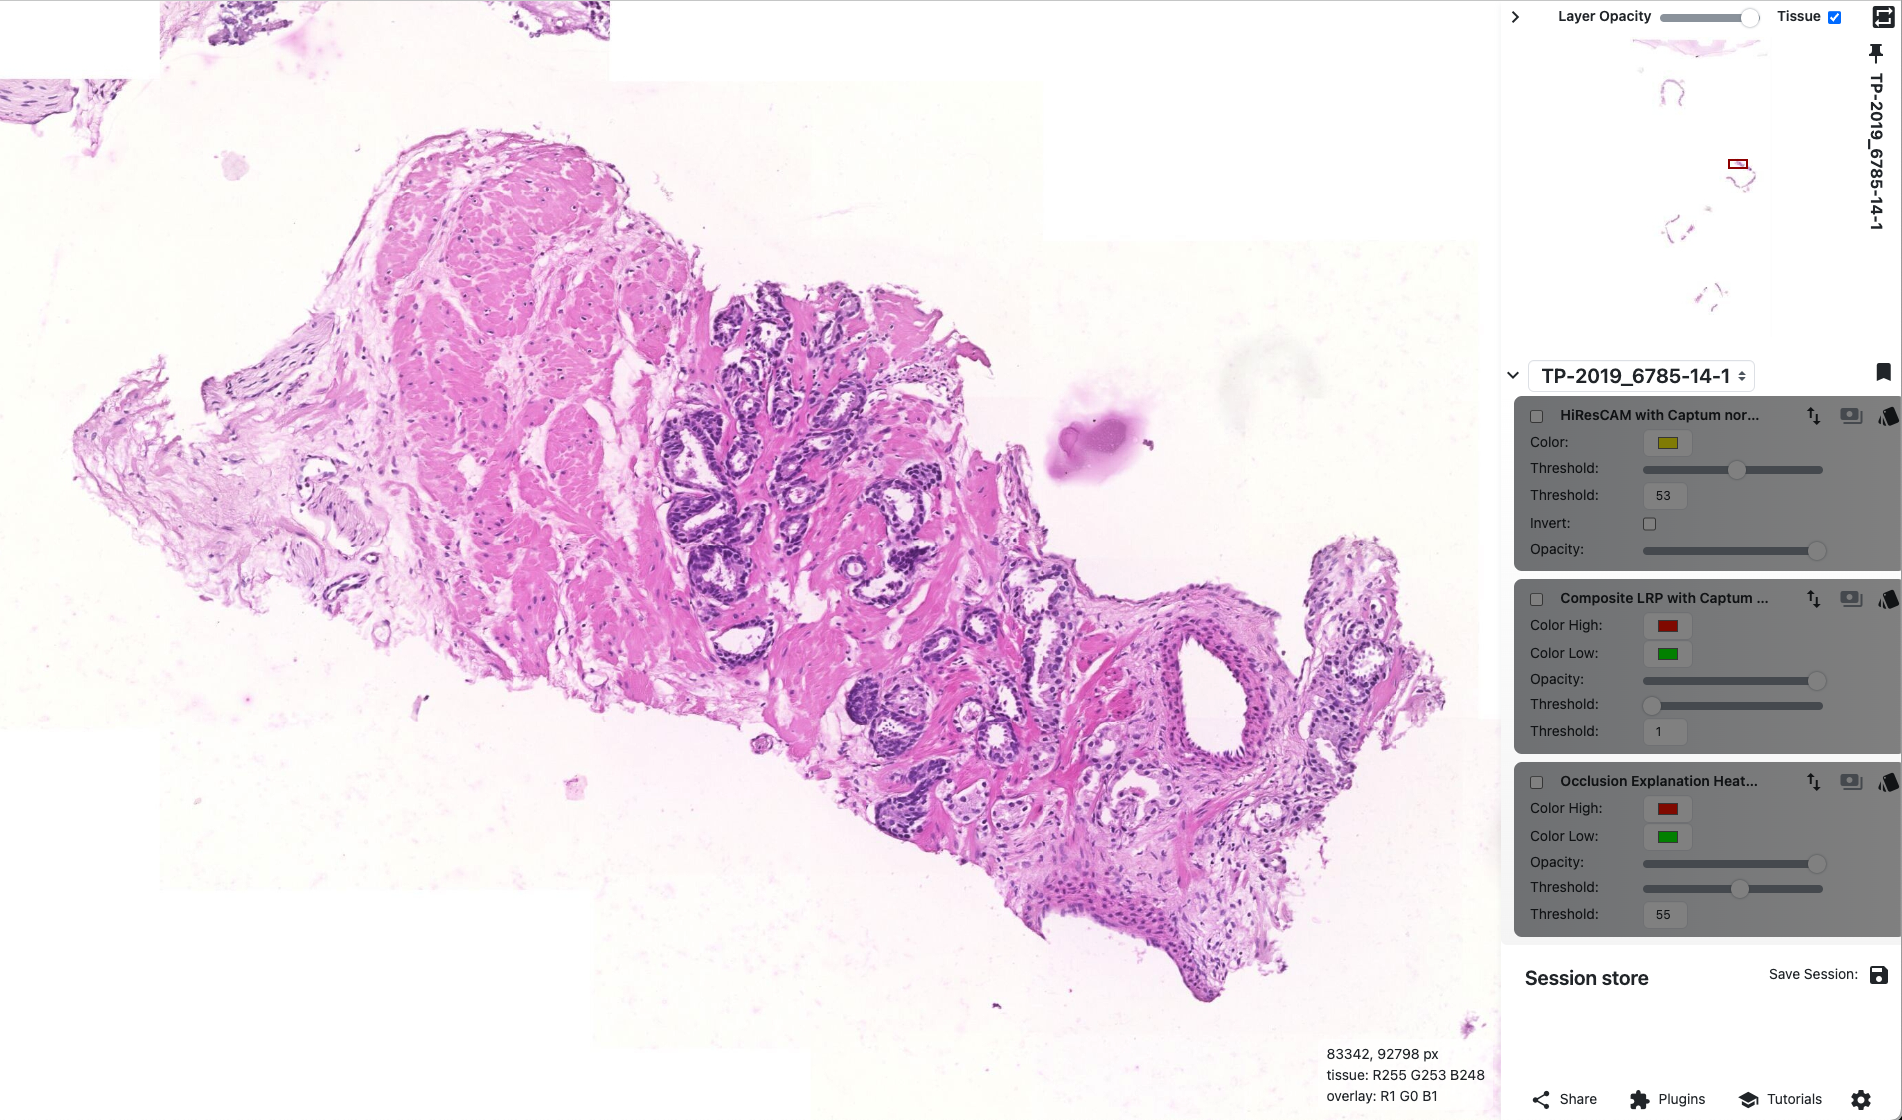
\includegraphics[width=\textwidth]{img/xopat.png}
    \end{minipage}
    \caption{xOpat [] WSI browser with a sample of prostate tissue. Histopathologist is able to move and zoom the tissue, allowing him to quickly navigate in the WSI. Having digitized copies allows for layering of arbitrary annotations on top of the WSI, providing great collaborative capabilities.}
    \label{fig:xopat}
    \end{center}
\end{figure}
\todo{Maybe add border?}

\subsection*{Decision Support System}

A computer system, which aids human to make a decision while performing a particular task is referred to as decision support system []. These systems are utilized across a wide array of applications, including high-stake environments such as investment banking [], autonomous driving [] or military and defense []. In digital histopathology, such systems are usually utilized to help with operational processes []. With deep learning in the spotlight of today's research, new possibilities emerge.

New systems could be utilized to enhance tissue diagnostic process by assisted diagnosis, or used to discover previously unrecognized features in large sets of data, incomprehensible by a single expert [].
%% https://pathsocjournals.onlinelibrary.wiley.com/doi/10.1002/path.5388
Random forests [], support vector machines [] and various neural network architectures [] are all attempts of such utilization. Those systems often provide real-time results and human-like performance, demonstrating that further research in this area can bring significant improvement to the contemporary processes [].

%% decision trees - https://www.researchgate.net/publication/363350224_Random_forest_modelling_demonstrates_microglial_and_protein_misfolding_features_to_be_key_phenotypic_markers_in_C9orf72-ALS
%% svm - https://www.ncbi.nlm.nih.gov/pmc/articles/PMC1924513/pdf/1471-2121-8-S1-S8.pdf
%% neural networks - https://arxiv.org/pdf/2312.02225.pdf
%%                 - https://www.sciencedirect.com/science/article/pii/S2666827021000992

\section{Deep Learning}
%% Brief intro to what is deep learning, methods and techniques? Common use cases of deep learning in digital histopathology.

Area of machine learning encapsulating neural networks is referred to as deep learning (DL). Methods and algorithms employed by DL achieve remarkable results across various domains, including computer vision [imagenet?], games [alphago], weather forecast [] and natural language processing [gpt].

Introduced in 1943 by McCulloch and Pitts [] with goal of creating a computational unit resembling a neuron in human brain, neural networks have come a long way to the prominent place they occupy today.

%% forecast - https://www.nature.com/articles/s41586-023-06185-3

\subsection*{Feed-forward Neural Network}

A multi-layer perceptron is a simple feed-forward neural network. It can be seen as a function $f$ that maps real-valued input vector \textbf{x} to a single value $\hat{y}$. As the name suggest, a multi-layer perceptron is organized into layers and each layer consists of its trainable weights and biases, commonly in form of a real-valued matrices. Additionally, each layer has its activation function\footnote{Heaviside step function was the first activation function to be used. This led to a number of problems [] and because of their importance, activation functions are vital part of research interest up to this day [].}, usually denoted as $\Theta$. Formula for a function $f_l$ computed by a layer $l$ with weights $w_l$, biases $b_l$ and activation function $\Theta_l$ is denoted as:

\begin{equation}
\hat{y_l} = \Theta_l(w_l \cdot x + b_l)
\end{equation}
where $\hat{y_l}$ is output of the layer $l$, or simply $f_l(x)$.



Even though ... shows that one hidden layer is all you need to essentially approximate arbitrary function, artificial neural networks often consists of multiple layers. The motivation is that each layer can be seen as if it captures certain abstractions or patterns from its input. Deeper layers can build more complicated patterns utilizing abstractions captured by previous layers. Figure \ref{fig:simple-mlp} depicts a simple multi-layered perceptron (MLP) with one hidden layer.

Deep learning aims to make networks weights and biases useful. Since a network computes a function $f$, with specific training, we can make network learn to approximate any desited function $f*$ within a certain tolerance.

To achieve this, training leverages large amount of data to adjust networks parametes to minimize difference between its and desired outputs. This process is typically performed iteratively using loss function, backpropagation, and traning algorithm such as stochastic gradient descent. More on neural networks training can be found in [].

%% goodfellow kniha

\begin{figure}[!h]
    \begin{center}
    \begin{minipage}{.75\textwidth}
      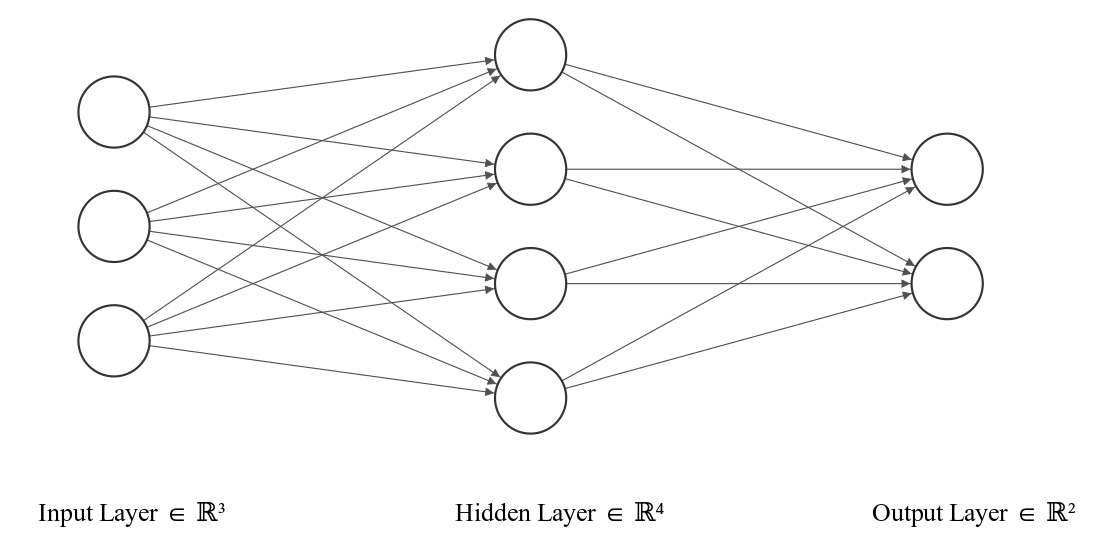
\includegraphics[width=\textwidth]{img/nn.png}
    \end{minipage}
    \caption{Architecture of a multi-layer perceptron with one hidden layer. Circles represent layer inputs. Edges represent layer weights. Biases are omitted for simplicity. Given a non-input layer L, if every unit has an incoming edge from all units in previous layer, we consider the perceptron to be fully-connected.}
    \label{fig:simple-mlp}
    \end{center}
\end{figure}

Despite MLP's demonstrating impressive results on tasks previously considered as impossible for computers, they come with some setbacks. Given they are fully connected, even small contemporary architectures such as ImageNET with multiple layers would have unimaginable number of trainable parameters. This led to development of new architectures, tailored to specific domain needs. Despite shift from using fully-connected layers only, MLP stood its ground and to this day, it is essential part of various state of the art neural network models [gpt, alexnet].

\subsection*{Convolutional Neural Network}
%% Architecture
Architecture introduced specifically to solve various computer vision problems adds two additional layer types --- convolutional and pooling. These layers help to capture features from input image, as well as reduce size of the network []. 
%% - https://arxiv.org/pdf/1511.08458.pdf

%% TODO: Why it suits them for image processing

\subsubsection{Convolutional Layer}

Convolutional layer works similar as to layers in a MLP. It utilizes learnable filters (alternatively called kernels) to search for patterns in its input.

Typically, a filter has significantly smaller dimensions compared to the input. Instead of interacting with whole input at once, as it is case for fully-connected layers, the filter is systematically slid across the input. Weights of a filter are convolved with the corresponding input data segments. This yields an activation map, which can be seen as a evidence for presence of a shape, detected by the filter in the input data.

When defining a convolutional layer, aside from filter shape, we need to supply two additional parameters, usually called \emph{padding} and \emph{stride}. Padding is used at the borders of the input feature map, to help prevent loss of information, where the filter could not be otherwise applied. Stride controls how much we shift the filter upon calculating one convolution. See Figure \ref{fig:cnn-convolution} for visualization.

\begin{figure}[!h]
    \begin{center}
    \begin{minipage}{0.75\textwidth}
      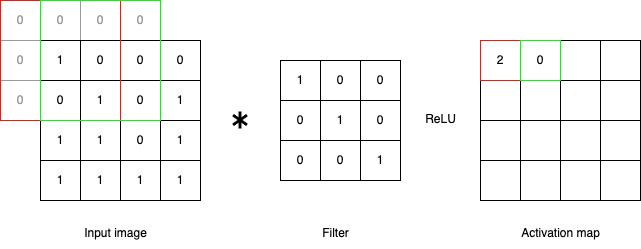
\includegraphics[width=\textwidth]{img/cnn-conv.png}
    \end{minipage}
    \caption{Example of simple calculation within convolution layer. Filter detects diagonal edge of lenght 3 pixels. Stride and padding are both set to 1 pixel and zero is used as the padded value. The result is passed through ReLU activation function.}
    \label{fig:cnn-convolution}
    \end{center}
\end{figure}

It is important to note, that a filter shares its weights with every input segment it attributes to. This gives us spatial in-variance -- meaning the filter is able to detect learned pattern at any position in the input features. Moreover, it drastically reduces the number of weights. Given $512$ input and output features, fully connected layers would need $262144$ weights. Simple $3x3$ filter needs $9$.

Traditionally, a convolutional layer consists of multiple filters. The idea is, that each filter is trained to activate upon seeing a different pattern. Given a one layer can detect multiple shapes, as outlined in section ..., it allows the deeper layers of network to combine simple patterns into more complex ones.

\subsubsection{Pooling Layer}

To prevent overfitting, pooling layers are employed to further distill patterns captured by a CNN. They progressively reduce size of the features, leading to reduced number of model parameters and computational complexity [].

A pooling layer is commonly placed after a convolutional one, iterating over its activation maps. It has its own filters and strides, however, the parameters are chosen more conservatively. Most of the time, filter is of size $2x2$ and stride is set to $2$, such that the pooled sectors do not overlap. It is reported that having a filter of size greater than 3 will most likely lead to loss of model's performance, since such granularity would hide more of the detected features [].

\begin{figure}[!h]
    \begin{center}
    \begin{minipage}{0.5\textwidth}
      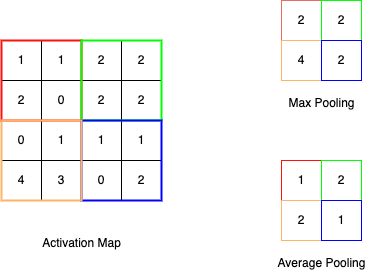
\includegraphics[width=\textwidth]{img/cnn-pool.png}
    \end{minipage}
    \caption{Example of both max and average pooling layers. Both have filters of size $2x2$ and stride set to $2$, resulting in no overlap during computation. Notice, that since each $2x2$ region is mapped to a single value, the new activation mask has quarter the features of the original.}
    \label{fig:cnn-pooling}
    \end{center}
\end{figure}
%%

    \chapter{Prostate Cancer Detection Setting}

According to the Masaryk Memorial Cancer Institute, prostate cancer is the most common oncological disease amongst men in the Czech Republic, with around $8$ thousand new cases reported each year \cite{mmci-prostate-cancer}.
In the global context, experts estimate $1,276,106$ of new cases appeared solely in $2018$ \cite{world-prostate-cancer}.
To aid pathologists in tackling the ever-growing number of new cases, the RationAI team trained and tested a CNN on a dataset provided by Masaryk Memorial Cancer Institute.

This chapter briefly introduces prostate cancer, a contemporary approach to detecting malignant tissue, and finally, a dataset and RationAI's model for prostate cancer detection.

\section{Prostate Cancer}

Prostate cancer is a disease that causes rapid growth of cells in the prostate -- a male gland under the bladder.
This gland is responsible for producing seminal fluid that aids in the transport and nourishment of sperm.
The type of cancer attacking glandular tissue is called adenocarcinoma.

Doctors commonly diagnose prostate cancer amongst men after $50$ years of age, and the incidence rate keeps increasing with aging --- we detect nearly $60$\% presence in men over $65$.
The mortality rate per $100,000$ people varies worldwide, ranging from $3.3$ in Eastern Asia to $10.7$ in Central America. Diet, physical activity, ethnicity, and family history are all likely to influence cancer's development and progression.
Implications of prostate cancer are notable even if it does not result in death, as it affects one's quality of life due to potential urinary, bowel, and sexual dysfunctions.
In advanced stages, prostate cancer can spread beyond the prostate gland, affecting the bladder, rectum, or bones \cite{world-prostate-cancer}.
Given the high prevalence and potential for aggressiveness, early detection and effective management of prostate cancer are vital to improving outcomes and survival rates.

\subsection*{Gleason Patterns and Score}

To effectively detect and estimate the impact of adenocarcinoma spread in the prostate, in 1996, Donald Gleason presented a unified grading and scoring system.
Gleason's system gained acceptance in 1974 and is the most prevalent system doctors use today.
It categorizes the growth of cancer cells into distinctive patterns based on how much the cancerous tissue differs from healthy prostate gland cells, as shown in \myref{Figure}{fig:gp}.
Several patterns and their descriptions have been refined later; today, we differ between 9 patterns. Complete enumeration and description of patterns can be found in \cite{gleason-patterns}.

To calculate a Gleason score, the histopathologist determines the predominant and second most common Gleason pattern -- the final score is simply a sum of pattern category numbers. The International Society of Urological Pathology distinguishes between $5$ grades of prostate cancer. More on scoring and grading innuendos can be found in \cite{gleason-pattern-grading}.
In 2016, WHO refined the grading into so-called \emph{grade groups} \cite{who-grade-groups}.

\begin{figure}
    \begin{center}
    \begin{minipage}{1\textwidth}
      \frame{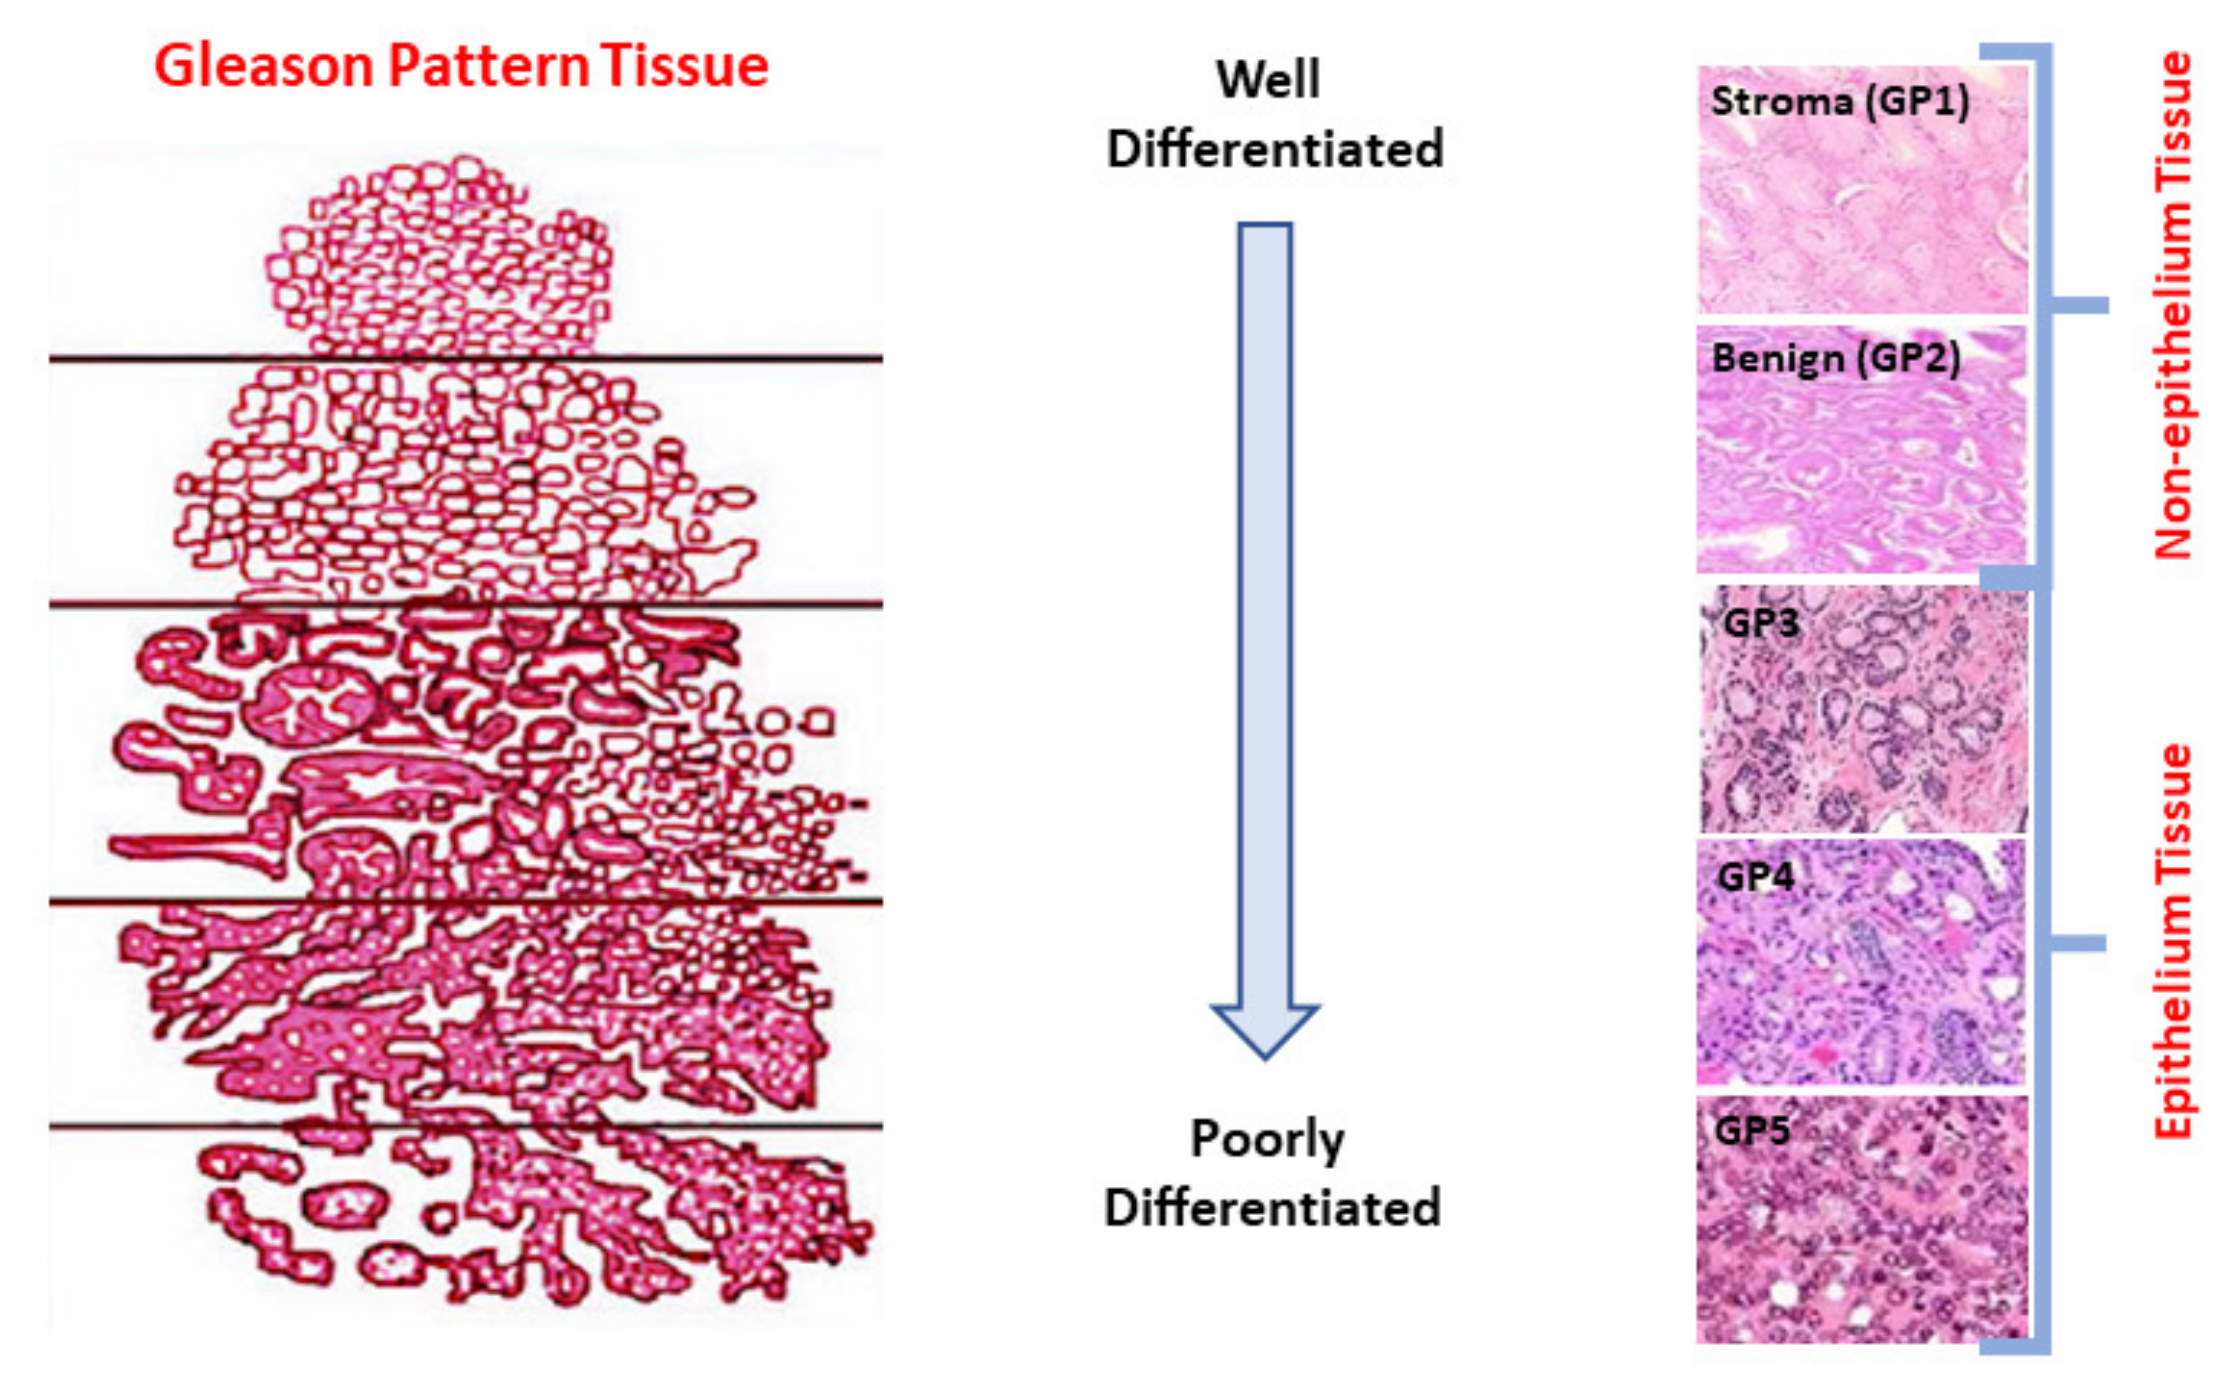
\includegraphics[width=\textwidth]{img/gp-classification.png}}
    \end{minipage}
    \caption{Example of Gleason Patterns ranked from $1$ to $5$. Pattern $1$ represents a healthy stroma --- ``cells and tissues that support and give structure to organs, glands, or other tissues in the body'', per definition from \cite{nci-stroma}. Pattern $5$ represents tissue with the highest risk of cancer. Sourced from \cite{gleason-pattern-description}}
    \label{fig:gp}
    \end{center}
\end{figure}

\section{Dataset}\label{sec:dataset}
\todo{level + priblizeni}
Masaryk Memorial Cancer Institute provided the RationAI group with a pseudonymized hematoxylin/eosin-stained WSIs dataset.
Each WSI contains $3$ to $5$ biopsies and is stored as a MIRAX uncompressed PNG of size $105,185 \times 221,772$ pixels.
The dataset is stratified into training and test split, containing $264$ WSIs with cancer, $436$ without, $37$ WSIs with cancer, and $50$ without, respectively \cite{gallo}.
\myref{Table}{tab:who_grade_distribution} shows the WHO grade group distribution.
\todo{case vs. slide}
\begin{table}
\centering
\ra{1.2}
\begin{tabular}{@{} l l l @{}}\toprule
WHO Grade Distribution & Training split & Test split \\ 
\midrule
Grade 1         & 38 cases            & 5 cases      \\
Grade 2         & 31 cases            & 1 case       \\
Grade 3         & 16 cases            & 1 case       \\
Grade 4         & 9 cases             & 1 case       \\
Grade 5         & 10 cases            & 2 case       \\
\bottomrule
\end{tabular}
\caption{WHO grade distributions for Training and Test split of prostate WSI dataset.}
\label{tab:who_grade_distribution}
\end{table}

\todo{in matejs paper, there is something about the distribution negatively affecting some results.}
To mark cancerous areas, domain experts manually annotated areas of WSIs containing adenocarcinomas -- annotations are polygons encapsulating cancerous regions.
Because processing the whole WSI at once is computationally expensive, we tile the WSIs to decrease memory requirements.
Each WSI is split into overlapping tiles of size $512 \times 512$ pixels.
An overlap of $256$ pixels is used between two consecutive tiles to counter the possibility of severing critical patterns.
Such tiling is a well-established approach used industry-wide, as per [].

WSIs contain several biopsies with blank spaces in between them.
To chisel out only relevant parts of WSI, any tile with less than $50$\% of its area covered by tissue is discarded from training and testing dataset splits.
Consequently, while all WSIs have the same size, their usable tile count differs.

\subsection*{xPOI Dataset}\label{xpoi-dataset}

The WSI dataset is vast, and to verify that models trained by the RationAI group focus on the important morphological features, \cite{gallo} sampled a small subset of this dataset to present to a domain expert upon model's evaluation.
This dataset consists of $461$ tiles.\todo{check actual count and write something in there}.

\section{Model}\label{model}

A model trained by RationAI to perform cancer detection in tiled WSIs is a modified version of the well-known CNN architecture VGG16, introduced in \cite{vgg16}.
\myref{Figure}{fig:rationai-vgg16} portrays the full model breakdown.

Loosely paraphrasing \cite{gallo}, the model aims to solve the following problem: \emph{Classify tiles according to the presence/absence of cancer in their central square area of $256 \times 256 $ pixels. Presence is determined by whether the central square overlaps with the annotation from the domain expert}. The model achieves a notably good score on the test split, reaching $100$\% slide-level prediction accuracy --- meaning the model correctly determines whether a WSI contains cancer for each of the test WSIs.

However, blindly trusting the model in such a high-stake environment, as cancer detection undoubtedly is, based on accuracy, is not enough.
To verify that the model bases its decisions on relevant features, Gallo et at.\todo{fix smaller font} conducted an additional experiment, presenting a subset of the dataset from \myref{Section}{sec:dataset} including regions of models' interest to a domain expert.
Using the technique described in the \myref{Subsection}{occlusion}, Gallo et al. annotated those data to display models' areas of interest.
The domain expert concluded that the model focuses on critical morphological features \cite{gallo} on which human pathologists would base their decisions.

\begin{figure}
    \begin{center}
    \begin{minipage}{0.75\textwidth}
      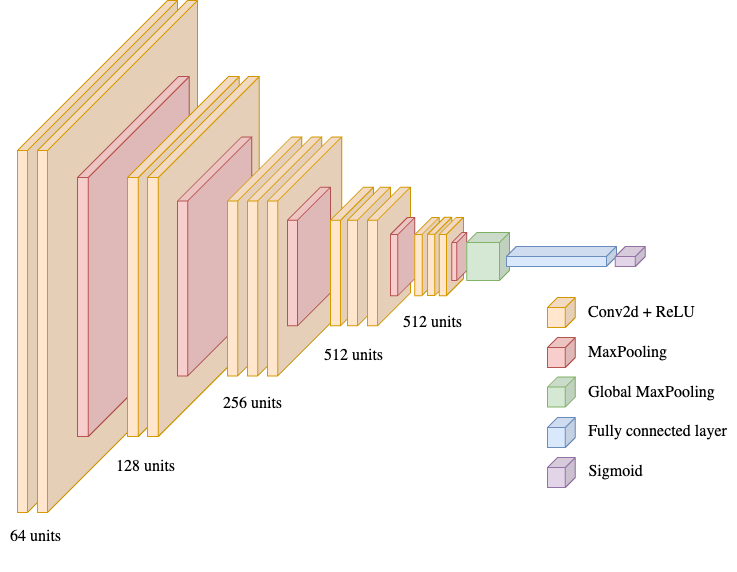
\includegraphics[width=\textwidth]{img/nn-arch.png}
    \end{minipage}
    \caption{Architecture of Prostate Cancer Binary Classifier model utilized by the RationAI group. The model is based on VGG16, introduced by Simonyan and Zisserman in \cite{vgg16}. They originally trained their VGG16 model to classify $1000$ classes from the ILSVRC dataset \cite{ilsvrc} and utilized three FC layers before applying softmax on the last one. RationAIs' solution places global max pooling before a single FC layer, reducing each of the $512$ pooled activation maps to a single value. Sigmoid is applied to the output of the FC layer to squish the raw value in the range $(0, 1)$. This can be seen as an extension of the logit model, with condensed activation maps as independent variables. Therefore, we can interpret the final output as a probability of pro-cancer markers in a given tile's central $256 \times 256$ pixel square.}
    \label{fig:rationai-vgg16}
    \end{center}
\end{figure}


    \chapter{Explaining Neural Networks}

This chapter covers an introduction to the growing field of explainable artificial intelligence.
We start with a short overview of the field itself, followed by motivation for understanding the decisions of neural networks, alongside a brief overview of legal obligations placed on decision support systems by the European Union.
We continue with an overview of several explainability methods suitable for our domain and task.
This will serve as a foundation for the next chapter, where we evaluate selected methods against our benchmark.

In contemporary literature, several terms are used to address the incomprehensibility of ML models. Arrieta et al. distinguish the following idioms \cite{arrieta-taxonomy}:
% TODO - make actual definitions

\begin{enumerate}
    \item Understandability: Characteristic of a model to make a human understand its function without any need for explaining its internal structure or the algorithmic means by which the model processes data internally
    \item Comprehensibility: Ability of a learning algorithm to represent its learned knowledge in a human-understandable fashion 
    \item Interpretability: Ability to explain or to provide the meaning in understandable terms to a human.
    \item Explainability: An accurate proxy of the decision maker and comprehensible to humans.
    \item Transparency: A model is considered to be transparent if, by itself, it is understandable.
\end{enumerate}

They further emphasize the distinction between interpretability and explainability -- interpretability, closely coupled with transparency, are inherent and passive characteristics of a machine learning model.
On the contrary, explainability is an initiated action taken to clarify the models' internal details.
Both can be seen as means to achieve understandability -- how a human can make sense of decisions made by the model \cite{arrieta-taxonomy}.


\section{Need for understandability}\label{sec:need-for-xai}

State-of-the-art neural network models are often products of billions of parameters \cite{arrieta-taxonomy}.
The term "black-box" models has been coined to highlight their complex internal mechanics.
In a crusade for ever-better performance and accuracy, models inherently grow in size and depth.
Increasing size and complexity raise concerns in the research community and the general public about whether these networks can be trusted and used responsibly \cite{arrieta-taxonomy, xai-survey}.

\subsection*{Spurious Correlations}

Distrust does not stem only from a lack of insight into the model's internal reasoning.
In certain cases, the seemingly flawless performance of machine learning models may result from a systematic bias in training and evaluation data.
A commonly used example is an experiment by Ribeiro et al. in \cite{xai-husky}, where they purposely trained a logistic regression classifier to distinguish between wolves and husky dogs.
The dataset was compiled such that images of wolves consistently featured snow in the background, whereas those of huskies did not.
This led the classifier to base its decisions on the presence of snow in the picture rather than the animal itself. 

\myref{Figure}{fig:horse-tag} presents a more unintentional example.
One can see that a \emph{capable} model may arrive at the desired output despite disregarding features on which humans would base their decision-making process. 

Instances such as these demonstrate that the understandability of a decision support system isn't just an issue for the end-user.
It's also advantageous for the model's development cycle.
Gaining insights into the factors influencing the model's decisions allows us to evaluate if its reasoning aligns with our expectations responsibly --- and take measures if not.

\begin{figure}[!h]
    \begin{center}
    \begin{minipage}{1\textwidth}
      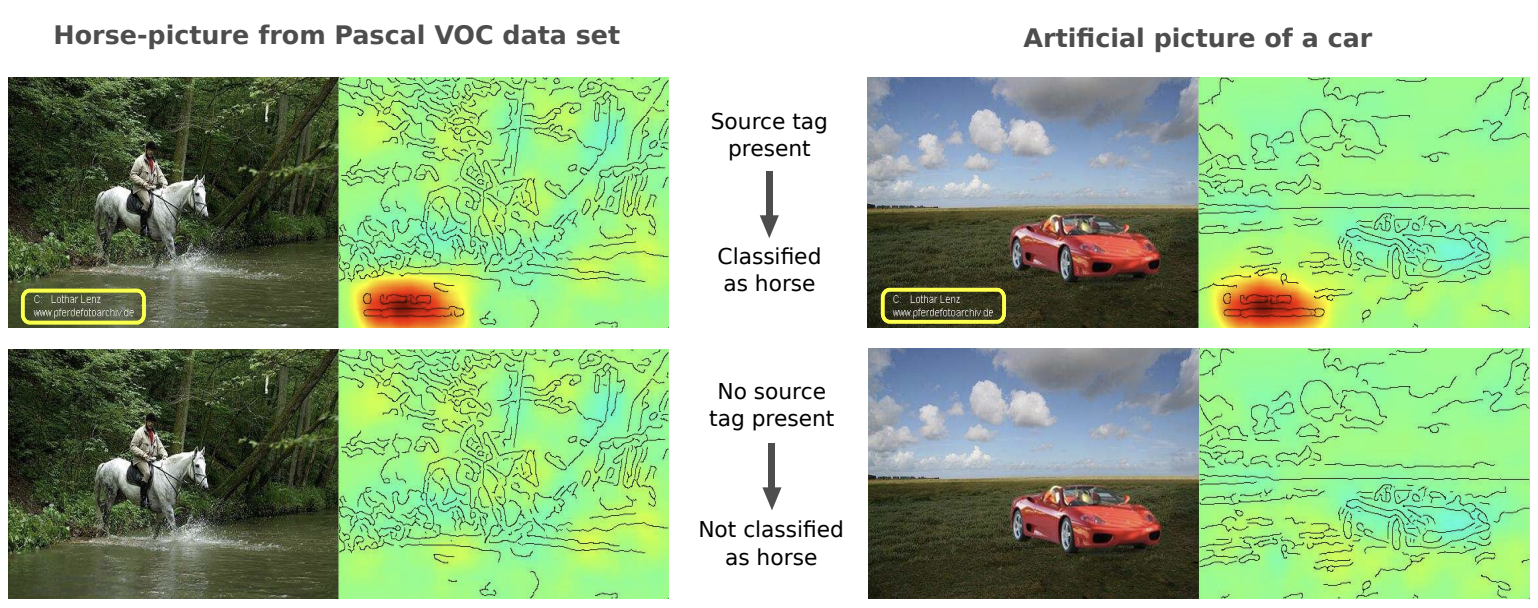
\includegraphics[width=\textwidth]{img/horse-tag.png}
    \end{minipage}
    \caption{Experiment conducted by Samek et al. in \cite{xai-horse}. Their model was trained on the PASCAL-VOC dataset \cite{pascal-voc}. After the training, they found the presence of so-called \emph{spurious correlation}. Pictures of horses are classified solely on whether the bottom-left corner of an input image contains a source tag. If the source tag is manually added to an otherwise correctly classified image of a car -- the model changes its prediction, and the image is classified as a horse instead. Picture taken from \cite{xai-horse}.}
    \label{fig:horse-tag}
    \end{center}

\end{figure}

\subsection*{Explainability in medical domain}

Such spurious correlations and the black-box tag make clinicians skeptical about integrating AI in healthcare.
A recent survey by GE HealthCare \cite{ge-healthcare-survey} concludes that out of 2000 clinicians participating, $58$ percent do not have overall trust in AI systems, and $44$ percent of respondents believe that the AI-based systems are biased.
Achieving the trust of both clinicians and patients is crucial to enabling industry-wide utilization of machine learning-based systems.

\subsection*{Legal obligations for AI explainability in the European Union}

Given certain applications, understanding the model is not only a moral obligation.
In 2016, the European Union included the \emph{right to explanation} within the General Data Protection Regulation (GDPR).
Specifically, Articles 13 and 14 give individuals the right to receive ``meaningful information about the logic involved'' when they are a part of an automatic decision-making process.
This challenges the industry and implies we must take adequate measures to fully integrate DSSs based on deep learning.
More on what Articles 13 and 14 mean for AI is to be found in a paper by Goodman and Flaxman \cite{xai-gdpr}.

Another piece of legislation from the European Union is anticipated to be implemented in May or June of 2024.
\emph{AI Act} introduces a series of regulations for machine learning-based AI systems.
The legislation is notably more detailed and exhaustive than Articles 13 and 14 of the GDPR, yielding mixed responses from domain experts.
While the full implications are yet to be seen, it already imposes several restrictions on what must be met before deploying machine learning models.
One section specifically targets high-risk AI systems.
It states that ``providers must build for human oversight, incorporating human-machine interface tools to ensure systems can be effectively overseen by natural persons.''.
Several aspects of the models' life-cycle are also revised, ranging from training datasets to technical documentation.
A comprehensive overview of the article is beyond the scope of this thesis and is summarized by Veale and Borgesius in \cite{xai-ai-act}.

\section{Explainable Artificial Intelligence}

The rapid development of deep learning models and scarcity of trust among users, combined with an attempted regulation, call for tools and methods that allow us to understand and justify outputs of otherwise opaque systems.
To shed light on the internal processes of machine learning models, a sub-field of Explainable Artificial Intelligence (XAI) covers a range of techniques to make models more understandable while preserving their performance and effectiveness.
XAI techniques enable humans to build trust and manage machine learning-based decision support systems, a crucial part of integrating systems based on deep learning.
The exact borders of the field are not firmly set, and the notion of what it means to explain a model is an ongoing matter of discussion \cite{xai-survey}.

\todo{find citations, forgot to write down}

Throughout this thesis, `XAI' will refer specifically to the subfield dedicated to advancing understandability in AI, while 'explainable artificial intelligence' will denote the attribute of machine learning models that enables a certain level of understandability. Arietta et al. \cite{arrieta-taxonomy} describe explainable artificial intelligence as: ``Given an audience, an explainable Artificial Intelligence is one that produces details or reasons to make its functioning clear or easy to understand.''.

The field of XAI distinguishes between two means of making artificial intelligence understandable:
\begin{enumerate}
    \item Using transparent model: Models based on linear regression or decision trees are inherently interpretable -- therefore understandable by themselves. We can derive how they came to the given conclusion by looking at their parameters.
    \item Using post-hoc explainability methods: When dealing with neural networks, we gain little insight into how they operate by simply inspecting their weights. Therefore, we must implement auxiliary methods, which simplify and distill the reasoning of networks so that, according to the definition --- we get a clear and easy-to-understand explanation. Post-hoc explainability methods can be further divided into two subgroups -- global methods explaining the model as a whole and local methods, focused on internal reasoning behind prediction for a particular input sample.
\end{enumerate}

In recent years, a plethora of both global and local post-hoc explainability methods have been introduced to help grasp the decision process of deep neural networks. Post-hoc methods can be further divided into two groups. Model-specific methods are designed to explain only models with specific features and capabilities -- such as attention-based models or convolutional neural networks. On the contrary, model-agnostic methods can explain arbitrary machine learning models \cite{arrieta-taxonomy}.

\section{Making CNN's Understandable}

For convolutional neural networks, the industry-wide standard is to visually highlight parts of an image, which are considered \emph{important} to the model. The result of such visualization is commonly referred to as a \emph{saliency map}, class activation map, or attribution map. There is no consensus on terminology, and we will use the term saliency map to describe any heatmap that identifies regions considered important by a post-hoc method. 

The following subsections overview several explainability methods we benchmark in \myref{Chapter}{experiment}.
We deliberately chose methods not covered in previous work by RationAI's team in \cite{gallo, krajnansky-grad-cam}.
Popular methods such as LIME, Deconvolution, or $\epsilon$-LRP  were either computationally too expensive or produced sub-par results, which are not deemed satisfactory \cite{gallo}.
When choosing methods for this thesis, we focused on the observation of Gallo et al. in \cite{gallo} --- methods, which tend to attribute continuous regions of tiles scored higher in the previous benchmarks.
Therefore, we focused on methods specifically created for explaining CNNs, leveraging their spatial memory ability.

\subsection{Occlusion}\label{occlusion}

Occlusion is a model-agnostic method from a family of so-called input perturbation-based methods.
Occlusion computes the saliency map by systematically covering square parts in the input image and observing the change in models' prediction confidence on the perturbed image.
Intuitively, we expect that when we cover (occlude) an important part of the input image, the confidence of our classifier drops.
On the contrary, when we cover a region without relevant features, the output should not differ too much from the output for the non-perturbed image.
The visual example can be seen in \myref{Figure}{fig:occ-saliency}. This approach gives us a rough (depending on the patch size) heatmap of input feature saliency.

An experiment conducted by Gallo et al. \cite{gallo} shows that this method produces semantically correct saliency maps on the xPOI Dataset.
Occlusion detects several recognized Gleason patterns.
Sadly, occlusion comes with high computational complexity and resource utilization.
For our use case, using an occlusion patch of $55 \times 55$ pixels and stride of $27$ pixels, the method needs 289 forward passes to compute the saliency map for a single tile.
On a machine with $8$ cores, $16$GB of RAM, and $48$GB of GPU memory capacity, occlusion needs approx. $2$ seconds and $40$GB of GPU memory to generate a single saliency map.
Recall Section Y and our approach to WSI tiling.
In our test set, slide size varies from 400 to 4000 tiles per slide.
Omitting auxiliary saliency map processing, occlusion takes anywhere from $13$ to $130$ minutes to explain a single WSI.

\begin{figure}[!h]
    \begin{center}
    \begin{minipage}{1\textwidth}
      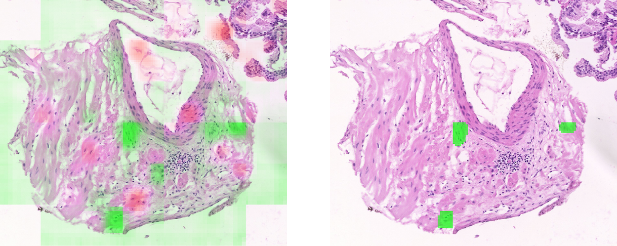
\includegraphics[width=\textwidth]{img/occlusion.png}
    \end{minipage}
    \caption{Sample of prostate tissue with Occlusion generated saliency. Green areas denote parts important for the model, while red parts signify not pro-cancerous areas. Since saliency maps are generated on a tile level, they are further composed, and overlapping areas are averaged to produce slide-level saliency maps. The sigmoid function is applied to saliency maps before combining, as is reported in \cite{gallo} to positively affect the smoothing and stability of the explanations. We do not use produced saliency maps as they are since they tend to be very noisy, as depicted in the left picture. Instead, the saliency map is thresholded to include only the most salient features, as depicted on the right, with a threshold of $55$ percent.}
    \label{fig:occ-saliency}
    \end{center}
\end{figure}

\subsection{CAM \& GradCAM}\label{subsec:cam}
\todo{they are the same thing up to a constant, so overview the GradCAM method here}

Zhout et al. \cite{cam} show that introducing a GAP layer to a convolutional neural network has a welcome side-effect --- aside from regularization during training, it enhances network localization capabilities, despite being trained on image-level labels only --- without specifying wherein the input the object of interest resides.
Their proposed method, called Class Activation Mapping (CAM), is used to visually highlight regions of input image used by the CNN to predict certain class $c$.
This model-specific method works only with networks with a GAP (or GMP) layer as the intermediate between the last convolutional layer and the final fully connected layer.
If a network satisfies this property, it is said to have a ``CAM architecture''.
The original paper uses a network with a convolutional layer before global pooling.
Our model features there a pooling layer instead.
This difference does not affect the results overviewed in the following paragraphs, and we will model them using a convolutional layer as per the original paper. 

Intuitively, CAM is a weighted sum of activation maps of the last convolutional layer.
To formalize, consider a network with convolutional layer $L$ with $K$ activation maps $A^1, A^2, \ldots, A^K$, followed by a GAP layer and a single fully connected layer.
In the fully connected layer, we fix neuron denoting class $c$, for which we want to compute a saliency map.
Recall \myref{Equation}{gap}, and that GAP reduces the value of each activation map $A^k$ to a single value $a^k$ --- the average of the activation map.
The score of the network for class $c$ is then calculated as
\begin{equation}\label{eq:gap-score}
    y^c = \sum_{k=1}^K w_{ck} a^k.
\end{equation}

To construct a class activation map for class $c$, we reverse-engineer the calculation of $y^c$. The saliency map is constructed out of individual mappings, and mapping for spatial element $(S^c_{\text{CAM}})_{ij}$ is calculated as a weighted sum of activation maps $A^k$
\begin{equation}\label{eq:cam}
    (S^c_{\text{CAM}})_{ij} = \sum_{k=1}^K w_{ck}  A^k_{ij}.
\end{equation}
To obtain saliency map $S^c_{\text{CAM}}$, we calculate mappings for all pairs $i, j$.
The saliency map $S^c_{CAM}$ directly indicates the importance of the respective spatial locations.
If pooling layers are present in the network, they lead to activations in the last convolutional layer having smaller dimensions than the input grid.
This is addressed by up-sampling the $S^c_{\text{CAM}}$ to the size of the original input image.

The authors point out that this method is particularly useful for networks featuring the GAP layer.
They claim that using GMP instead leads to the method pointing out the single most discriminatory location instead of all of them, as is the case for GAP.
While this has been largely confirmed by their experiment on the ILSVRC dataset \cite{ilsvrc}, we believe that the method is worth considering for our use case.
Models employed in the experiment by Zhou et al. \cite{cam} are trained to distinguish between $1000$ classes, with their last convolutional layer having $1024$ units.
This configuration suggests a roughly one-to-one relationship between the activations produced by the network and the classes it aims to identify.
In our setting, the last convolutional layer has $512$ units to identify one class --- we posit that even though we eventually only extract the most discriminative location from each activation map, having $512$ units should still yield robust localization performance.
Our belief is supported by the fact that upon inspection of the weights of the fully connected layer of the model described in \myref{Section}{model}, $267$ out of $512$ weights are positive --- meaning corresponding activations are pro-cancerous.

Unlike CAM, GradCAM \cite{grad-cam} is a model-agnostic method that can explain various CNN architectures without needing a global pooling layer.
The idea is that since the convolutional layer holds spatial information about its activations, we can highlight the important ones using partial derivatives of the score $y^c$.

We will use the same setting as for \myref{Equation}{eq:cam}, with $L$ being a fixed convolutional layer of our network with $K$ units whose activation maps are $A^1, A^2, ..., A^K$.
GradCAM computes importance weight $i_{ck}$ for feature map $A^k$ as the average of partial derivatives of $y^c$ with respect to individual activations of $A^k$ \cite{grad-cam}
\begin{equation}\label{grad-cam-weights}
    i_{ck} = \frac{1}{|A^k|} \sum_{i=0}^H \sum_{j=0}^C \frac{\partial y^c}{\partial A^k_{ij}}.
\end{equation}

We substitute $i_{ck}$ for $w_{ck}$ in \myref{Equation}{eq:cam} and compute a weighted combination of activations and their respective importance to obtain a saliency map.
$\operatorname{ReLU}$ is applied over the weighted activations to get only positive values advocating for important features with respect to class $c$ \cite{grad-cam}
\begin{equation}
    (S^c_{\text{GradCAM}})_{ij} = \operatorname{ReLU}(\sum_{k=1}^K i_{ck} A^k_{ij}).
\end{equation}
Authors of GradCAM took the inspiration for using $\relu$ from Deconvolution and Guided Backpropagation, both post-hoc methods already covered in \cite{gallo}.
In case the saliency map $S^c_{\text{GradCAM}}$ is smaller than the input grid, we up-sample it as in the case of $S^c_{\text{CAM}}$.

GradCAM has been previously covered in \cite{hruska-grad-cam, krajnansky-grad-cam, bajger-grad-cam}, but as far as we are concerned, this method was not evaluated using a quantitative benchmark similar to one from \cite{gallo}. Moreover, as shown in \cite{bajger-grad-cam}, for our model, GradCAM saliency maps are identical to the ones generated by CAM, up to a constant factor of ${1}/{|A^k|}$.
\todo{rewrite this section about previous results}

\subsection{GradCAM++}
\todo{The function needs to be smooth (exp) so the 2nd and 3rd derivative are not 0 -- then it is NOT the same thing as CAM/GradCAM}

GradCAM++ \cite{grad-cam-pp} is another gradient-based model-specific method to spatially attribute convolutional layer features for a given class.
Like GradCAM, this method leverages gradients flowing through the network to assess individual activations' importance while adressing several of GradCAMs' imperfections.

Chattopadhyay et al. \cite{grad-cam-pp} observed that if multiple occurrences of a class of interest $c$ are present in the input image, the localization capabilities of GradCAM worsen.
According to the authors, this stems from using unweighted partial derivatives in \myref{Equation}{grad-cam-weights}.
If there are multiple occurrences of class $c$, different feature maps may get activated, resulting in a diluted and faded saliency map.
They proposed a generalized solution that is equivalent in terms of computational performance.
First, they encode the importance weight $i_{ck}$ from \myref{Equation}{grad-cam-weights} as
\begin{equation}\label{eq:grad-cam-pp-weights}
    i_{ck} = \sum_i^H \sum_j^W \alpha^{ck}_{ij} \relu(\frac{\partial Y^c}{\partial A^k_{ij}}).
\end{equation}

Then, they derive a method for expressing the gradient weights $a^{ck}_{ij}$ for all spatial locations in all activation maps.
They substitute weights from fully connected layer in \myref{Equation}{eq:gap-score} for importance weights $i_{ck}$ from \myref{Equation}{eq:grad-cam-pp-weights}, yielding
\begin{equation}\label{eq:grad-cam-pp-score}
    Y^c = \sum_{k=1}^K \left( \sum_{i=0}^H \sum_{j=0}^W \alpha^{ck}_{ij} \relu(\frac{\partial Y^c}{\partial A^k_{ij}}) \right) \left( \sum_{a=0}^H \sum_{b=0}^W A^{k}_{ab} \right)
\end{equation}
where $Y^c$ is a score $y^c$ put through the exponential function. To express a weight $\alpha^{ck}_{ij}$, we need to take a partial derivative w.r.t. $A^k_{ij}$ twice. After that, we can rearrange the terms to obtain
\begin{equation}
    \alpha^{ck}_{ij} = \frac{\frac{\partial^2 Y^c}{(\partial A^k_{ij})^2}}{2\frac{\partial^2 Y^c}{(\partial A^k_{ij})^2} + \sum_{a=0}^H \sum_{b=0}^W A^{k}_{ab} \left( \frac{\partial^3 Y^c}{(\partial A^k_{ij})^3} \right)}.
\end{equation}

All that is left is to plug this expression back into \myref{Equation}{eq:grad-cam-pp-weights}.
This gives us the importance weights for activations, and the saliency map $S^c_{\text{GradCAM++}}$ is computed the same way as $S^c_{\text{GradCAM}}$.
Thanks to the additional coefficient $\alpha^{ck}_{ij}$ for respective partial derivative, authors claim that all spatial coordinates corresponding to instances of class $c$ in the input data will be highlighted with equal importance in the resulting saliency map.

As shown in \myref{Subsection}{subsec:cam}, two different methods can produce the same saliency map.
To avoid adding a third one, we derive the particular values for importance weights $i_{ck}$.
The full derivative is presented in \myref{Section}{sec:grad-cam-plus-plus-weight-derivation} and yields, for $A^k_{ij}$ being the highest activation in unit $k$.
\begin{equation}
    i_{ck} = \frac{1}{2 + A^k_{ij}w_{ck}} \relu\bigl(\exp(y^c)w_{ck}\bigr).
\end{equation}
As a result, only activation maps corresponding to positive weights --- therefore, patterns detected as pro-cancerous --- are present in the final saliency map.
We lack rationale about the term $A^k_{ij} w_{ck}$ in the denominator, as more profound activations will receive a smaller importance weight.
Nevertheless, we have shown that for our architecture, GradCAM++ produces saliency maps that differ from CAM and GradCAM.
The extent to which the activation maps will differ is not easy to estimate, and we will include GradCAM++ in evaluation in \myref{Chapter}{experiment}.


\subsection{HiResCAM}\label{sub:hirescam}

HiResCAM, introduced in \cite{hires-cam}, is another gradient-based model-agnostic method that builds upon GradCAM's success.
The first step is the same as for GradCAM++ --- we need to compute partial derivatives of $y^c$ with respect to activation map $A^k$.
Instead of condensing the importance of the activation map to a single value, we arrange the partial derivatives into a grid and perform a pairwise multiplication of this grid with the respective activation map.
We compute the grid of partial derivatives for all activation maps $A^k$, and
\begin{equation}
    (S^c_{\text{HiResCAM}})_{ij}
        = \sum_{k=1}^K \frac{\partial y^c}{\partial A^k_{ij}} A^k_{ij}.
\end{equation}

Draelos and Carin \cite{hires-cam} arrived at a similar observation as in the case of GradCAM++ that GAP-ing the partial derivatives in \myref{Equation}{grad-cam-weights} leads to blurred feature maps. 
They believe that taking element-wise multiplication better reflects how models ``see" the input image.
This way, individual activations are scaled according to their partial derivative before being channel-wise summed up to form the final saliency map.

In addition to the method, the authors present proof of HiResCAM's capabilities.
The proof demonstrates that for convolutional networks ending in one fully connected layer $L$, HiResCAM guarantees to visually highlight all parts of the input image that increase class score $y^c$, given we compute the saliency map for the convolutional layer preceding $L$ \cite{hires-cam}.
Unfortunately, the proof does not cover our model introduced in \myref{Section}{model}.
While the model ends in one fully connected layer, it is separated from the last convolutional layer by an intermediate global max pooling operation, which reduces each feature map to a single value.
This breaks down the proof's assumption that we can extract spatial information from the feature maps in the FC layer, since such information will be destroyed in the GMP operation. 

The authors also show that given a model with CAM architecture employing GAP, saliency maps generated by HiResCAM collapse maps of the CAM method.
This does not hold for models using the GMP layer.
For our model, the partial derivative of $y^c$ with respect to $A^k_{ij}$ will be $w_{ck}$ iff $A^k_{ij}$ is the largest activation in $A^k$, and zero otherwise.
\todo{Elaborate on this one}
Therefore, the resulting activation map reflects only the most significant activation from each unit.
This differs from saliency maps produced by CAM and GradCAM++, which do not discriminate against individual activations that do not contribute to the model's output but are evidence for a detected pattern.
We believe that HiResCAM could better resemble how the Occlusion method produces the saliency maps since occluding features, albeit detected but not contributing to the output score because of GMP, should not produce a high saliency for the given region.

\subsection{ScoreCAM}

\todo{add what is the baseline}
To bridge the gap between perturbation-based and gradient-based methods, Wang and Wang \cite{score-cam} introduced ScoreCAM to tackle GradCAM's flaws from different perspectives.
Unlike it is the case for previous CAM-based methods, ScoreCAM does not rely on partial derivatives to compute the saliency.
Instead, authors rely on a so-called increase in confidence, which is, given input $x$, baseline $x_b$, and activation $A^k$, defined as:
\begin{equation}
    c^k = f\bigl(x \odot \operatorname{upscale}(A^k)\bigr) - f(x_b)
\end{equation}
where $\operatorname{upscale}$ is a function that resizes activation map $A^k$ to the input grid size and scales it to range $[0, 1]$.
We get a score indicating how much network confidence changes if we only supply areas of the image where filter $F^k$ found a pattern it is trained to detect.
We calculate the final saliency map using the respective increase in confidence as our weight for convolutional layer activation maps, yielding
\begin{equation}
    (S^c_{\text{ScoreCAM}})_{ij} = \relu\biggl(\sum_{k=1}^K c^k A^k_{ij}\biggr).
\end{equation}

%As a result, we eliminate the dependency on partial derivatives.
%According to the conducted experiments in \cite{score-cam}, ScoreCAM can locate multiple objects within the same activation map, something considered harder to achieve due to our utilization of the GMP layer.
% Authors mention that saliency maps computed by ScoreCAM are more "focused" than the ones computed by GradCAM++.
% While having focused saliency maps is a desired property, comparing results visually and drawing conclusions is considered anecdotal evidence, and proper quantitative assessment must be done [].

\subsection{AblationCAM}

Another gradient-free method, AblationCAM, introduced in \cite{ablation-cam}, utilizes ablation analysis to compute the importance of activation maps.
AblationCAM computes how an individual activation map $A^k$ contributes to the final score $y^c$ by "removing" it from the score computation and observing a drop in models' confidence.
The influence of the removal of feature map $A^k$ to the final score is defined as
\begin{equation}\label{eq:ablation-cam-importance-weight}
    d_{ck} = \frac{y^c - y^c_k}{y^c}
\end{equation}
where $y^c_k$ represents an output of the model, for which the activation $A^k$ is zeroed out.

Similar to Occlusion and input features, if we remove activations important to the network when assessing the presence of class $c$, the score $y^c$ should drop. To obtain the final saliency map, we compute the ablation weights for the layer of interest, yielding the following equation
\begin{equation}
    (S^c_{\text{AblationCAM}})_{ij} = \relu(\sum_{k=1}^K d_{ck} A^k_{ij}).
\end{equation}

\subsection{Layer-Wise Relevance Propagation}

While Occlusion estimated feature importance by observing changes in output and CAM-based methods utilized spatial information in the convolutional layers, Layer-Wise Relevance Propagation (LRP) \cite{lrp} takes a different approach.
Given an output score of the network, LRP utilizes several types of propagation rules to redistribute the score from the output layer down to the input pixels.
The idea is that we can look at how individual features contribute to the output of the network --- each feature value is weighted and sent to the upper layer across the whole network, ultimately contributing to the final class score.
In a reverse fashion, we can compute the importance of the input pixels \cite{lrp}.

To describe this procedure, assume that $i$ and $j$ are two neurons in consecutive layers, so there is a connection from $i$ to $j$. 
The process of propagating relevance $R_j$ from $j$ to $i$ is captured by the following generic propagation rule \cite{lrp}
\begin{equation}
    R_i = \sum_j \frac{z_{ji}}{\sum_k z_{jk}} R_j
\end{equation}
where $z_{ij}$ models to which extent neuron $i$ contributed to neuron $j$'s activation.
The extent $z_{ij}$ is derived by various rules, further described in \cite{lrp}.
The choice of rules is largely left to experimentation, however, Montavon et al. in \cite{lrp} provide a blueprint for choosing layers when working with VGG-16 based network.

The main building block is the LRP-$0$ rule, where the extent
\begin{equation}
    z_{ji} = y_i w_{ji}.
\end{equation}
Parameters $y_j$ and $w_{ji}$ stand for neurons output and weight, respectively, as defined in \myref{Section}{section:dl}.
\todo{are those really parameters?}

According to the observation of Montavon et al. in \cite{lrp}, using solely LRP-$0$ leads to very noisy explanations.
To tackle the noise, we add a small positive term $\epsilon$ to the denominator --- $\epsilon$ will absorb weak and contradictory contributions, preserving only the salient scores. 
As a result, we typically get less noisy explanations.
Gallo et al. used LRP-$\epsilon$ rule exclusively in \cite{gallo}.
However, such explanations were still deemed scattered and noisy.
To further enhance produced explanations, we can use LRP-$\gamma$ rule to favor positive contributions by using a coefficient applied only to the positive weights:
\begin{equation}
    z_{ji} = {a_j \cdot (w_{ji} \cdot \gamma w_{ji}^+)}.
\end{equation}
The $\gamma$ rule draws from the $\epsilon$ rule and keeps the $\epsilon$ term in the denominator.
Figure \ref{fig:lrp-montavon} shows how multiple rules can be composed to visually enhance explanations.

\begin{figure}[!h]
    \begin{center}
    \begin{minipage}{1\textwidth}
      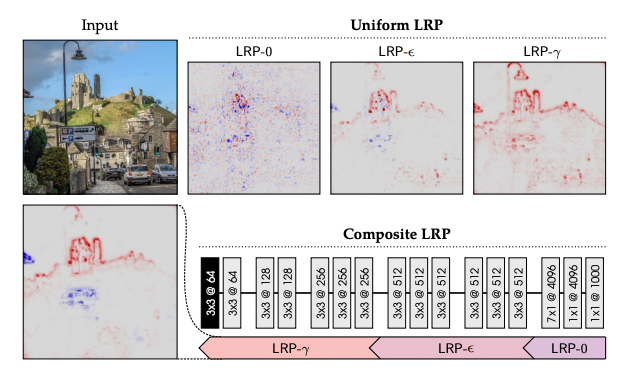
\includegraphics[width=\textwidth]{img/lrp-montavon.png}
    \end{minipage}
    \caption{Image show explanation results after different combinations of rules are applied. Notice that combining multiple rules yields a visually more coherent saliency map. According to Montavon et al. in \cite{lrp}, using LRP-$0$ in the upper layers is beneficial to combat the entanglement of different concepts represented by the network. LRP-$\epsilon$ in the middle layer helps to propagate only the most salient activations, while LRP-$\gamma$ in the lower layer ensures uniform relevance spread. Image taken from \cite{lrp}.}
    \label{fig:lrp-montavon}
    \end{center}
\end{figure}
    \chapter{Benchmark}

This chapter consists of three sections. First, we tackle the current problem of high computational resources utilization by occlusion-based saliency -- by measuring time and GPU memory it takes for a method to compute explanation. In the second part, we establishing quantitative benchmark, choosing suitable metrics alongside brief reasoning and evidence behind our choice. We compare methods introduced in Section N.M against Occlusion. We combine qualitative metrics capturing desired properties of explainability methods, alongside improved and refined metrics from original paper by Gallo et al [6]. In the last part, we conduct a human evaluation, where we present result of explainability methods to domain expert.

\section{What makes a good explanation?}

\emph{Unfortunately, “explainability” is a nebulous and elusive concept that is hard to target.} []
\newline
% https://arxiv.org/pdf/2209.00366.pdf

\noindent

Contemporary research does not provide a unified approach to measuring "goodness" of an explanation.  There are attempts to propose a set of properties a good explainability method should fulfill, but they are not aligned [2, 3]. What is more, some studies even present contradictory results, rendering objective conclusions even more challenging [4, 5]. According to Doshi-Velez [], "the field is crowded with evaluation methods, and there is no consensus on which are the “right” ones. Much less, there is not even agreement on which criteria should be evaluated". The challenge lies in the absence of ground truth for an explanation, and therefore we have no objective measure of grading the explanations []. However, through careful choice of metrics, we can reason that given audience and use-case, certain explainability method is sufficient. To avoid so-called "anecdotal evidence", we need to carefully pick our metrics, so that we ensure that explanation is:

% doshi How to Evaluate Explainability? – A Case for Three Criteria
% A Benchmark for Interpretability Methods in Deep Neural Networks

\begin{enumerate}
    \item Performant: This is the main bottleneck of current solution of Occlusion-based saliency. Without reasonable performance, we do not care how good a method is, since it cannot be utilized for practical purposes.
    \item Faithful: Ideally, we want to ensure that the explainability method only highlight the relevant parts of input.
    \item Useful: We need the explanations to be presented to domain experts in such way, that it is understandable for for them. If they do not understand the explanation, it is of little value. 
\end{enumerate}

\section{Computational complexity}

The main problem of the existing approach to generate explanations in the required time.

\subsection*{Time efficiency}

In order for the method to actively assist pathologist, the explanation needs to be computed fast enough to not disrupt his workflow. The main caveat of the current solution untilizing occlusion is that it takes too long. We let each method fully explain averagely-sized slide from test set. Each run is conducted 3 times, to make sure the result is not influenced by any momentarily factors. Results are presented in Table ...

\subsection*{GPU utilization}

Modern GPU's offer possibility of multiple processes performing computations on the same instance. For production deployment, this is important factor. High GPU utilization for single method can negatively affect number of parallel processes and therefore raise costs of production deployment. Since neural networks are generally expensive in terms of computational power, their usage inevitable leads to increase in carbon emissions. Since sustainability is a hot topic, it is wise to consider this aspect for future deployment and development.

\section{Quantitative evaluation}

This section covers use of several widely used metrics capturing desired traits of explainability methods.

\subsection*{Faithfulness}

Common approach to assess whether explainability method marks the relevant part of input is to perturb the image such that we remove those marked features, then backfill those area with certain fixed value -- similar to how occlusion estimates the importance. However, there are studies indicating that simply removing those features may not be correct, since the perturbed input can contain certain artifacts, leading to a distribution shift. This may affect the plausibility of such metrics, since we cannot tell whether the increase/drop in model's confidence is caused by distribution shift, or the features were really important [ROAR].

In paper by Gallo et al., methods suffering from potential artifact introduction were used to measure the faithfulness. Notably, occlusion and DTD received the highest scores, aligned with observation by Hsieh et al. -- that such metrics may favor methods, which rely on the same mechanism when estimating importance on input features []. Moreover employed metrics (Causal Deletion [] and Area Over Perturbation Curve) did not produce aligned results.
% https://arxiv.org/pdf/2006.00442.pdf

To tackle the distribution issue, Hooker et al. [ROAR] present metric called Remove and Retrain (ROAR), which first removes the marked features, and then retrains the model on newly created dataset. While this method got widely accepted, it brings significant drawback in form of how computationaly exhaustive would this method be for our use-case. As ... shown, ROAR does not solve the problem of \emph{class information leakage} -- phenomenon, when the uniformly-valued mask itself reveals relevant class info through its shape [ROAD].

Rong et al. propose method building on foundations of ROAR, called Remove and Debias (ROAD). Instead of retraining the model, areas after removed features are imputed in such fashion that risk of class information leakage is reduced. For further reading and information theory behing imputation, refer to original paper [].

To evaluate performance of methods described in Section ..., we will iteratively remove features from the most important to the least (MoRF order). After each removal, missing features are imputed using noisy-linear imputer, to reduce class information leakage. We evaluate the metods at $10, 20, 30, 40, 50$ percents removed, as in the original paper. It is desired, that score should drop significantly as we start removing the features and the rate slows down as we approach the $50$\% border, as it signals that the important parts were removed as first. For evaluation, we used implementation from \emph{pytorch-gradcam} package.
% road

Since this method relies on sensitivity, we will only use positive tiles from test split of dataset from Section ....

\subsection*{Localization}
% localization
Faithfulness metric tells us, how well the explainability method important locations. Now we want to make sure, that these location resemble something a pathologist would use to decide, wheter there is cancer in the tissue or not. To measure how well a output of given method resembles pathologists annotation, Effective Heatmap Ratio (EHR) was used. This approach relies on bounding boxes, which encapsulates objects of interest. We argue, that it is not the best method to be used for our use case.

Given a bounding box, according to how EHR is calculated, it always favor methods which highlight larger areas of the image. This is not desired, as the bounding box only marks cancerous tissue -- the exact borders are difficult to find [Matej] and such annotion would likely vary pathologist from pathologist [].

\todo{Tu chcem ocitovat nieco o tom, ze patologovaia sa casto nezhoduju}

We will use technique called Weighting Game instead []. It build upon widely-employed Pointing Game metric [], which looks whether the most attributed pixel falls into the bounding box. Unlike pointing game, which gives us just binary information about the highest pixel, Weighting Game calculates ratio of the mass of the explanation within the bounding box with respect to total mass of the explanation. Unlike EHR, this does not disqualifies methods which highlight smaller parts of annotated area and and gives us very good measure, of how the explanation holds compared to the pathologist's annotation.

\subsection*{Usefulness}

It is almost impossible to determine usefulness of explanation by any quantitative metric, since how we perceive given explanation varies from person to person -- the audience is again a crutial part []. Luckily, we already know that solution based on occlusion proposed in [Matej] produces semantically correct explanations, which are of great use to the pathologist []. Therefore we will reuse metric from Subsection LOCALIZATION and we take $55$\% of most salient Occlusion result as our bounding box. Since such "annotations" do not represent ground truth, we do not perceive this metric as adding to the truthfulness of explanation method. Instead, it will serve as a guide for which methods we should present to pathologist, and we can measure how well will his former assessment of Occlusion stand against his new assessment of explainability methods introduced in Chapter XAI.

\subsection*{Robustness}
% max sensitivity
Another desired property is resistance against small perturbations. In order for explanations to be deemed trustful by clinicians, we need to be sure that the produced explnations are stable and not prone to adversarial attacks. Yeh et al. [] propose metric called Max-Sensitivity to measure how explanation changed when the input is exposed to insignificant (small) perturbations. This metric utilized Monte-Carlo sampling approach when generating explanations, and is computationaly expensive. Therefore the evaluation is performed only on the subset of test split data from Subsection USEFUL.


\section{Domain expert assessment}

This section presents qualitative evaluation of produced explanations by domain expert. We replicate experiment from []. What follows is assessment from Dr. Nenutil on how are explanations perceived from POV of a clinician.


  \bookmarksetup{startatroot}


  \addcontentsline{toc}{chapter}{Conclusion}
\chapter*{Conclusion}

\todo{future work TCAV, clustering}


  % % \appendix
\addtocontents{toc}{\protect\setcounter{tocdepth}{0}}

\renewcommand{\thechapter}{A}
\chapter{Appendix}

\section{GradCAM++ Importance Weights}\label{sec:grad-cam-plus-plus-weight-derivation}

Without the loss of generality, let us fix unit $k$ with the highest activation $A^k_{ij}$.
Since we utilize the GMP layer, all partial derivatives in \myref{Equation}{eq:grad-cam-pp-weights} will be zero, except for the one corresponding to the highest activation.
As a result, we can dismiss both sums, and the partial derivative weight becomes 
\begin{equation}
    i_{ck} = \alpha^{ck}_{ij} \relu(\frac{\partial Y^c}{\partial A^k_{ij}}).
\end{equation}
Authors already derived the activated score $Y^c = \exp(y^c)$ for us, and given the architecture of our model, the following set of equations holds:
\begin{equation}
\begin{aligned}
  \frac{\partial Y^c}{\partial A_{ij}^k}       &= \exp(y^c) \frac{\partial y^c}{\partial A_{ij}^k}     &&= \exp(y^c) w_{ck}     \\
  \frac{\partial^2 Y^c}{\partial (A_{ij}^k)^2} &= \exp(y^c) \bigl(\frac{\partial y^c}{\partial A_{ij}^k}\bigr)^2 &&= \exp(y^c) (w_{ck})^2 \\
  \frac{\partial^3 Y^c}{\partial (A_{ij}^k)^3} &= \exp(y^c) \bigl(\frac{\partial y^c}{\partial A_{ij}^k}\bigr)^3 &&= \exp(y^c) (w_{ck})^3.
\end{aligned}
\end{equation}

Plugging it all together, we get 
\begin{equation}
    \alpha_{ij}^{ck} = \frac{\exp(y^c) (w_{ck})^2}{2 \exp(y^c) (w_{ck})^2 + A^k_{ij} \exp(y^c) (w_{ck})^3} = \frac{1}{2 + A^k_{ij}w_{ck}}
\end{equation}
and subsequently
\begin{equation}
    i_{ck} = \frac{1}{2 + A^k_{ij}w_{ck}} \relu\bigr(\exp(y^c)w_{ck}\bigl).
\end{equation}

\pagebreak

\section{Convolutional Versus Pooling Layer for CAM-Based Methods}\label{sec:conv-vs-pool}

While it may seem natural to compute the saliency maps for the last convolutional layer, we decided to explore our options.

The final convolutional layer produces $512$ activation maps, each containing $32 \times 32$ activations.
If we upsample the weighted activation map $A^k$ to the size of $512 \times 512$ pixels, each spatial activation corresponds to a $16 \times 16$ part of the upsampled activation map.
If we use the last pooling layer instead, the dimensions are reversed, and individual elements of $16 \times 16$ pooled activation map will correspond to $32 \times 32$ pixels in the upsampled saliency map.
The production setting for Occlusion uses a patch of $55 \times 55$ pixels, with $27$ pixels stride.
We believe that the calculation of saliency maps for the pooled activations could closely resemble those produced by Occlusion.

While we have verified that saliency maps for the pooling layer are visually more similar to Occlusion than saliency maps for the convolutional layer, according to \cite{xai-anecdotal-evidence}, such an ``anecdotal'' conclusion is insufficient.
By applying the pooling operation, we condense the original activation map to $25$ percent of its original size, and this may lead to a loss of information when reconstructing the saliency map, undermining its faithfulness.
Thus, we conducted an additional experiment to compare both approaches using the faithfulness metric from \myref{Section}{sec:quant}.
The distribution of ROAD ratios is shown in \myref{Figure}{fig:road-conv-vs-pool}, and a visual comparison of both approaches is presented in \myref{Figure}{fig:conv-vs-pool}

Based on the results, we decided to continue with the saliency maps computed with respect to the pooling layer.
There is a negligible difference for CAM, and we posit the pooled saliency maps as more similar to Occlusion.
The same is true for HiResCAM; although the convolutional layer receives a much smaller ratio spread, the saliency maps tend to be more scattered and blurred.
For GradCAM++, using the convolutional layer is not an option.
Due to the inverse proportion between activation strength and the resulting importance weight, the less important regions are marked as more salient when the saliency map is computed for the last convolutional layer.
As we impute more of the area based on the saliency strength, the actual important regions are taken into account, and the model's score for perturbed images slowly decreases.
This is mostly tackled in the case of the pooling layer, as the more condensed activations seem to even out the indirect proportion. 
The difference for GradCAM++ regions imputed by the ROAD metric is shown in \myref{Figure}{fig:gradcampp-road-conv-vs-pool}.

\begin{figure}
    \begin{center}
    \begin{minipage}{1\textwidth}
      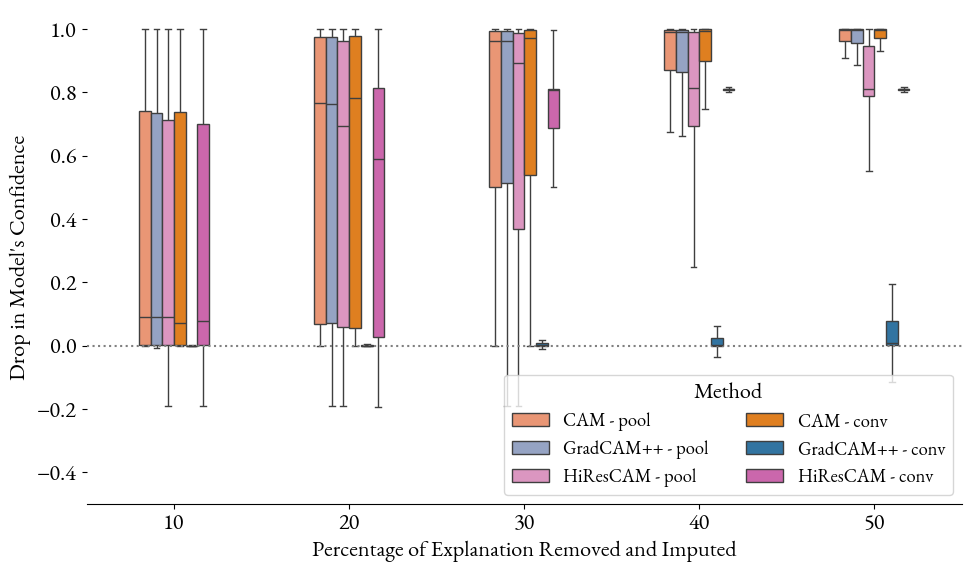
\includegraphics[width=\textwidth]{img/road-conv-vs-pool.png}
    \end{minipage}
    \caption{
    Comparison of ROAD ratios when attributing the last pooling versus the last convolutional layer.
    The CAM scores are almost the same, with the convolutional layer saliency maps being slightly more faithful according to our metric.
    HiResCAM achieves a significantly smaller spread when computing saliency maps with respect to the convolutional layer.
    However, the median is similar to its pooling layer counterpart.
    The largest difference comes for GradCAM++.
    We believe this is due to our finding in \myref{Subsection}{sub:gradcampp}, where activation strength is inversely proportional to the resulting importance weight.
    }
    \label{fig:road-conv-vs-pool}
    \end{center}
\end{figure}

\begin{figure}
    \begin{center}
    \begin{minipage}{0.5\textwidth}
      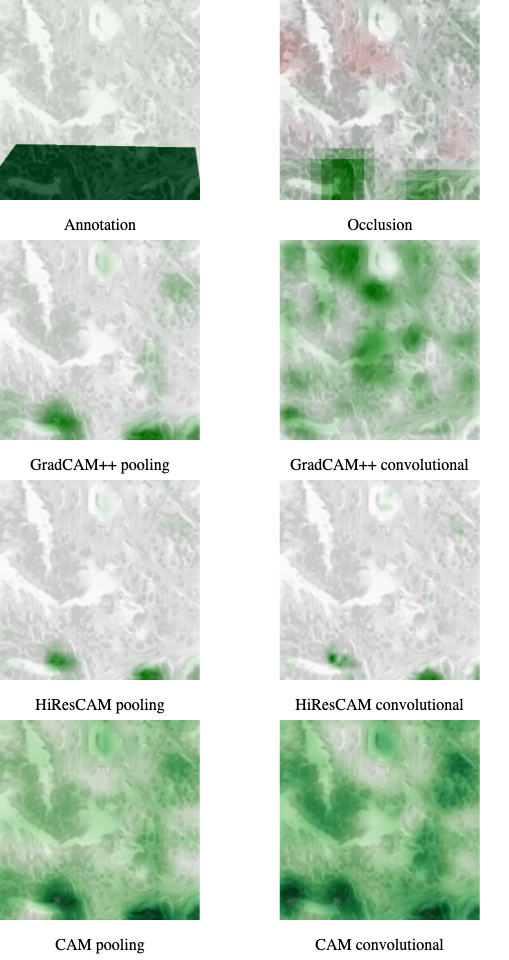
\includegraphics[width=\textwidth]{img/conv-vs-pool.png}
    \end{minipage}
    \caption{
    Visual comparison of saliency maps produced by CAM methods w.r.t. to the last pooling and the last convolutional layer of our model on a randomly selected tile.
    The underlying tile is shown in black and white to increase visual contrast.
    Note that Occlusion falls within the annotation boundaries, except for the top right corner.
    However, artifacts like this are removed using thresholding in the WSI browser.
    GradCAM++ is completely different when attributing the convolutional layer, focusing mostly on parts of the image that Occlusion and the annotation consider irrelevant.
    This changes once we compute the saliency maps w.r.t. the pooling layer.
    HiResCAM produces visually similar results, and despite producing similar results for this tile, the pooling saliency maps tend to cover larger and less scattered areas of the input tile.
    CAM is very liberal about the area covered, and the saliency maps are similar.
    However, the pooling one is easier to threshold because of the greater difference in saliency outside and inside the annotated area.
    }
    \label{fig:conv-vs-pool}
    \end{center}
\end{figure}

\begin{figure}
    \begin{center}
    \begin{minipage}{0.7\textwidth}
      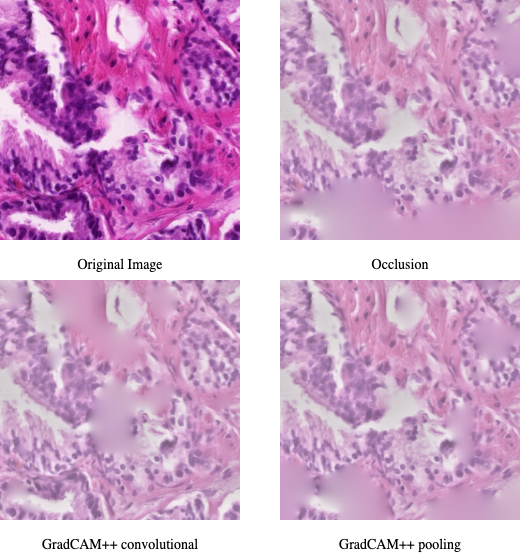
\includegraphics[width=\textwidth]{img/gradcampp-road-conv-vs-pool.png}
    \end{minipage}
    \caption{
    Visualization of different imputation results when we use the convolutional instead of the pooling layer for GradCAM++.
    On the original tile, the model accurately reports a confidence of $0.98$ for the presence of cancer.
    Both Occlusion and GradCAM++ w.r.t pooling layer accurately point to the relevant locations in the bottom of the tile, and the confidence on the perturbed tile drops to almost $0$.
    For GradCAM++ w.r.t. convolutional layer, the saliency map attributes different regions, and the confidence of our model on the perturbed image remains the same.
    We used \texttt{pytorch-grad-cam}'s implementation of visualizing the perturbed input, hence the discoloration.
    }
    \label{fig:gradcampp-road-conv-vs-pool}
    \end{center}
\end{figure}

\pagebreak

\section{Implementation}\label{sec:imple}

The source code of the benchmark, as well as the custom implementation of both CAM and HiResCAM, can be found in the \texttt{prostate-cancer} repository included in the supplementary materials. The source code is required to be run on the RationAI group's cluster, which has access to the test WSIs used for evaluation. Please visit the \texttt{README.md} file for installation and usage instructions. The \texttt{README.md} file also contains links to WSI with overlayed saliency maps available for inspection, given access rights issued by the RationAI group.

  \backmatter
  \printindex
  \begingroup
  \sloppy
  \printbibliography
\endgroup


\end{document}
